\chapter{IMPLEMENTATION AND DESIGN}

\sepfootnotecontent{fn:unity-engine}{[Footnote: What is the Unity engine]}

\sepfootnotecontent{fn:triple-a}{AAA (pronounced "triple A") games are an informal classification of video games distributed by major publishers and distinguished by large development and marketing budgets. In general, the term is used to represent the games that are supposed to achieve the highest standard of quality and content in video games.}

\sepfootnotecontent{fn:genshin-impact}{Genshin Impact (miHoYo, 2020). Video Game. Android, iOS, Windows, PlayStation 4, Playstation 5, Nintendo Switch.}

\sepfootnotecontent{fn:escape-tarkov}{Escape from Tarkov (Battlestate Games, 2017). Computer Game. Microsoft Windows.}

\sepfootnotecontent{fn:hollow-knight}{Hollow Knight (Team Cherry, 2017). Video Game. PlayStation 4, Nintendo Switch, Xbox One, macOS, Linux, Microsoft Windows.}

\sepfootnotecontent{fn:ghost-tale}{Ghost of a Tale (SeithCG \& Plug In Digital, 2016). Video Game. PlayStation 4, Nintendo Switch, Microsoft Windows, Xbox One.}

\sepfootnotecontent{fn:cuphead}{Cuphead (Studio MDHR Entertainment Inc., 2017). Video Game. PlayStation 4, Nintendo Switch, Xbox One, Microsoft Windows, macOS.}

\sepfootnotecontent{fn:undead}{\emph{Undead} beings are fictional characters represented by entities that were reanimated from death through supernatural means. Common representations of \emph{Undead} beings in popular media include \emph{Zombies}, \emph{Skeletons} and \emph{Vampires}.}

\sepfootnotecontent{fn:particle-vfx}{Footnote: What are particle-based visual effects}

\sepfootnotecontent{fn:death-stranding}{Footnote: What is Death Stranding}

\sepfootnotecontent{fn:core-gameplay-loop}{Footnote: What is the Core Gameplay Loop}

\sepfootnotecontent{fn:character-controller}{Footnote: What are CharacterControllers}

\sepfootnotecontent{fn:movement-drifting}{Footnote: What is movement drifting}

\sepfootnotecontent{fn:lock-on}{Footnote: What is Lock-On targeting}

\sepfootnotecontent{fn:colliders}{Footnote: What is a collider}

\sepfootnotecontent{fn:collider-overlapping}{Footnote: What is collider overlapping}

\sepfootnotecontent{fn:monobehaviour}{Footnote: What is a MonoBehaviour}

\sepfootnotecontent{fn:fixed-update}{Footnote: What is the FixedUpdate timestep}

\sepfootnotecontent{fn:rays}{Footnote: What are rays}

\sepfootnotecontent{fn:raycasts}{Footnote: What are Raycasts}

\sepfootnotecontent{fn:mecanim}{Footnote: What is the Mecanim system}

\sepfootnotecontent{fn:skeletal-rigs}{Footnote: What are skeletal rigs}

\sepfootnotecontent{fn:motion-sickness}{Footnote: What is motion sickness}

\sepfootnotecontent{fn:unity-prefabs}{Footnote: What are Unity Prefabs}

\sepfootnotecontent{fn:unity-gameobjects}{Footnote: What are Unity GameObjects}

\sepfootnotecontent{fn:transposing-and-composing}{Footnote: What are Transposing and Composing strategies}

\sepfootnotecontent{fn:observer-pattern}{Footnote: What is the Observer pattern}

% ============================================================================
% ============================================================================
% ============================================================================

\section{Overview (TO DO)}

In this section, we specify the details for each of the major decisions and systems for the implementation of an appropriate replica of the core elements of Dark souls with the additional aspect of an adaptive system that dynamically adjusts game difficulty to the profile of a player. We provide a detailed list of the requirements of our implementation, along with the motivation for the choice of each technology and game asset.

% About our implementation of Dark Souls "Core"
We specify the design and implementation of the gameplay mechanics and systems in Bright Souls, using a restricted set of the elements in the original game as a reference and comparing it to our previous analysis from section \ref{sec:analysis-dark-souls}.

% About our implementation of DDA

% Brief description of all subsections: Tools and Frameworks, Game Assets and Aesthetics, Gameplay Mechanics and Systems, Artificial Intelligence, Telemetry and Performance Tracking, Dynamic Adjustments


% ============================================================================
% ============================================================================
% ============================================================================

\section{Tools and Frameworks}

% Brief overview of tools used in the project, specify that we chose Unity, Cinemachine, Post Processing Stack, Aura Volumetric Rendering

In order to implement an appropriate replica of the main elements that compose Dark Souls, we first require a framework that can provide the tools to assemble and render 3D environments with high visual fidelity. Then, it is useful to have a set of utilities and ready-to-use systems to implement the functional aspects of the original game, such as a standardized Input System that can deal with multiple input devices, a set of definitions and functions to manipulate 3D Camera behavior and control and a physics engine that can detect and handle collisions for at least basic geometry such as bounding boxes. For these reasons, we chose \emph{Unity}\sepfootnote{fn:unity-engine} as our development platform as it contains most of the essential functionality we require, with the added possibility of extending and adapting the purpose of its editor to satisfy any additional needs.

% Motivation for using Unity3D
% - A complete framework that is widely used in the industry, and is able to achieve AAA quality products with current examples in the industry;

Unity is widely used in the video games industry, with a feature-rich framework that supplies game developers with tools to achieve AAA\sepfootnote{fn:triple-a} quality products. Some examples of successful games implemented under Unity include Genshin Impact\sepfootnote{fn:genshin-impact}, Escape from Tarkov\sepfootnote{fn:escape-tarkov}, Hollow Knight\sepfootnote{fn:hollow-knight}, Ghost of a Tale\sepfootnote{fn:ghost-tale} and Cuphead\sepfootnote{fn:cuphead}.

% - A concise integrated editor that can be used for map editor, project folder organization, game data management;
Unity offers a concise, integrated project editor that offers functionality such as level editing, files and folders structural organization, game data management, in-game and serialized component inspection, a visual editor for serialized animation state machines, configuration options for deploying platforms and architectures, a debug console and tools for generating offline light mapping data for scene rendering.

% - A general API that provides the tools to implement virtually any type of game;
Unity also defines a streamlined API so developers can implement their custom game code in \textsc{C\#}, providing access to reusable functionality libraries and systems such as the component-based \textsc{MonoBehaviour} API, the serialized data \textsc{ScriptableObject} API, the Input and UI systems and even the Editor package, which permits the developer to extend the built-in functionality of the Unity Editor to develop Quality of Life tools for improved creation workflows.

% - Possibility to deploy in multiple platforms (Windows, Linux, macOS) with minimal changes in source code;
It is also possible to deploy Unity projects to multiple platforms such as Windows, Linux, macOS, PlayStation, Nintendo Switch and Xbox with minimal changes in code, as Unity's standardized API and builtin \textsc{IL2CPP} compiler translates Intermediate Language code into automatically generated \textsc{C++} code, which is then compiled into a native binary for each target platform.

% - Possibility to import free and paid assets from the Unity Asset Store for 3D Models, Animations, Sounds, UI Elements, Shaders, Post-Processing Effects, Visual Effects;
However, one of the key factors behind the choice of Unity as a platform was the possibility of including free and paid assets from the \emph{Unity Asset Store}, a digital platform for the distribution and acquisition of game assets such as 3D Models, Animations, Sounds, 2D UI Elements, Shaders, Post-Processing Effects and Visual Effects. Without this, it would be impossible for the authors to develop a game that would be sufficient to even remotely resemble the qualities of a AAA game such as Dark Souls. By acquiring and importing high-quality game assets into the project, it was possible to focus on the design and development of game systems, while also having AAA quality assets as a resource to work with.

% - Possibility to import plug-and-play APIs and systems such as Cinematic Camera behavior controllers, Third person Movement Controllers and Universal Input Device Managers that can be easily integrated into the project and development workflow;
% - Possibility to import and integrate multiple development tools that are tailored to the specific needs of the product being developed, such as data serialization utilities, map editor utilities, telemetry and database management tools and visual effect creation tools;
As for the implementation and reuse of infrastructural development tools and game systems, the Unity development team has in recent years made relevant effort towards modularized, plug-and-play systems with the \emph{Packages} system. The Packages system defines a streamlined workflow for importing game assets, editor utilities and engine functionalities, where it is possible to individually import packages that are specific to the requirements of a Project. For the scope of this work, one relevant example would be the \textsc{Cinemachine} package, which contains functionality and tools for manipulating 3D cameras with sophisticated behaviors, real-time configurable properties based on lenses for real-world cameras, and pre-configured implementations of common functionality for cameras in video games.

% - Authors had previous familiarity with the engine from personal and professional experience;
The final deciding factor for the choice of Unity as a development platform was the previous personal and professional background of the authors with the engine, having implemented a wide variety of 2D and 3D Games, VR Serious Games and data visualization tools under Unity. The familiarity with the provided APIs, along with the knowledge of how to achieve a steady and concise workflow permitted the authors to plan a robust architecture and select the appropriate tools to implement the core features of Dark Souls with an acceptable quality in comparison to the original game.

% ============================================================================
% ============================================================================
% ============================================================================

\section{Game Assets and Aesthetics}

% 3D Models, animations and sound assets were selected based on trying to replicate the same general 'feel' of Dark Souls
The assets for the implementation contained within this work were elected with the objective to serve as resources to attempt to replicate the general aesthetics of Dark Souls. Therefore, as a basis criteria for the selection of used assets, we use the brief analysis in section \ref{sec:analysis-dark-souls} as a reference to explore options in the Unity Asset Store within the \emph{'Dark Fantasy'} thematic subcategory.

% Fantasy Dungeon
First, we require a set of 3D models to assemble a playable 3D environment that satisfy the aesthetics of the 'Dark Fantasy' genre. For this purpose, we elected the asset pack \emph{Fantasy Dungeon} -- a collection of 3D models with a 'Ruined Castle' theme. The overall aesthetics and theme of this aspect pack appropriately resemble the sense of 'abandonment' in the original game. When considering functionality aspects, this pack contains modular 3D objects and pieces that can be easily assembled into a playable environment. Furthermore, the asset pack also contains pre-assembled scenes with appropriate lighting and optimized meshes, which were adapted to fit the requirements of our implementation.

% Figure: Assets used in setting up the environment
\begin{figure}
    \caption{A selection of screenshots from pre-assembled scenes using the 3D assets from the Fantasy Dungeon asset pack.}
    \begin{center}
        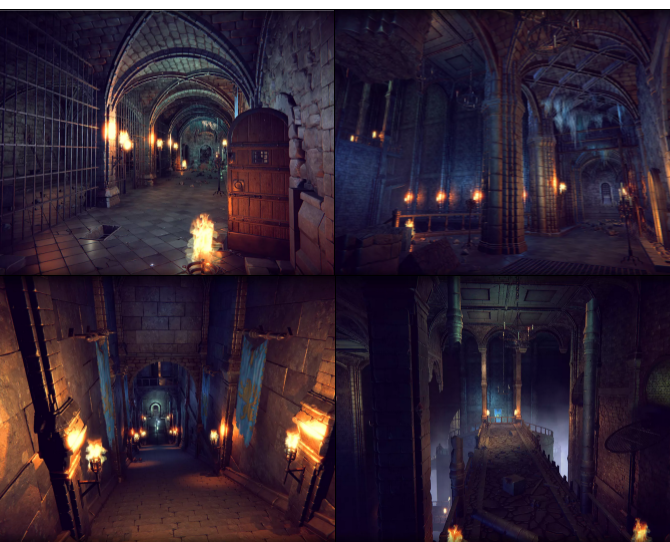
\includegraphics[width=24em]{figures/fig-environment-assets.png}
    \end{center}
    \legend{Source: Collation of screenshots performed by the authors from images captured from the original Unity Asset Store website pages for the \emph{Fantasy Dungeon} Unity asset.}
    \label{fig:environment-assets}
\end{figure}

% Then, we need 3D models for the Characters, The Blacksmith: Characters, Skeleton Zombies and Longsword Animset Pro

In sequence, we require 3D models to represent the playable character and any non-playable entities the player would be able to interact with. Regarding the non-playable entities, we attempt to implement enemy agents comparable to the enemies presented in the early levels of Dark Souls. Most of the enemies in these early sections of the original game are \emph{Undead}\sepfootnote{fn:undead} beings named \emph{'The Hollow'}, which are represented by creatures with decomposed skin and a dehydrated body that resemble the popular representation of \emph{Zombies}. In the original game, \emph{The Hollow} can be seen wearing a variety of attire, including ragged clothes, armored pieces such as cuirasses, pauldrons and helmets, bare skin or even without flesh in their bodies in the form of \emph{Skeletons}.

In addition to the requirement of being in harmony with the aesthetics of the original game, we also used as a criteria for the selection of enemy character models the requirement of serving a specific purpose in enemy behavior design and encounter design. Each enemy agent in our game should have a specific set of actions which can complement the actions of other enemies in a combat encounter. Therefore, we define enemy role archetypes based on the enemies seen in the initial levels of Dark Souls: the \emph{Ghoul}, the \emph{Archer}, the \emph{Swordsman} and the \emph{Assassin}.

Therefore, for the representation of enemy characters that satisfy our aesthetic and design requirements, we elected the asset packs \emph{Skeleton Zombies}, \emph{Longsword Animset Pro}, \emph{Modular Skeleton Archer}, \emph{Modular Skeleton Rogue} and \emph{Skeleton Humanoid}, all of which contain 3D models representing stereotypes of Zombies and Skeletons that resemble the enemies seen in the early stages of Dark Souls, while satisfying the roles we defined for the design of enemy agents in our implementation.

Another motivation for the selection of these asset packs was their compatibility with the \textsc{Mecanim}\sepfootnote{fn:mecanim} system, which standardizes \emph{skeletal rig}\sepfootnote{fn:skeletal-rigs} definitions for animations in humanoid characters in the \textsc{Unity} engine. When compatible with this system, character models can be used in combination with most animations that can be found in the \textsc{Unity Asset Store}, which provides the possibility of choosing from a wide collection of animation sets for multiple purposes, including animations for weapons wielded by the enemy characters we designed for our implementation.

% Figure: Assets used for character models
\begin{figure}
    \begin{center}
    \caption{A mosaic portraying the 3D character models in Bright Souls.}
        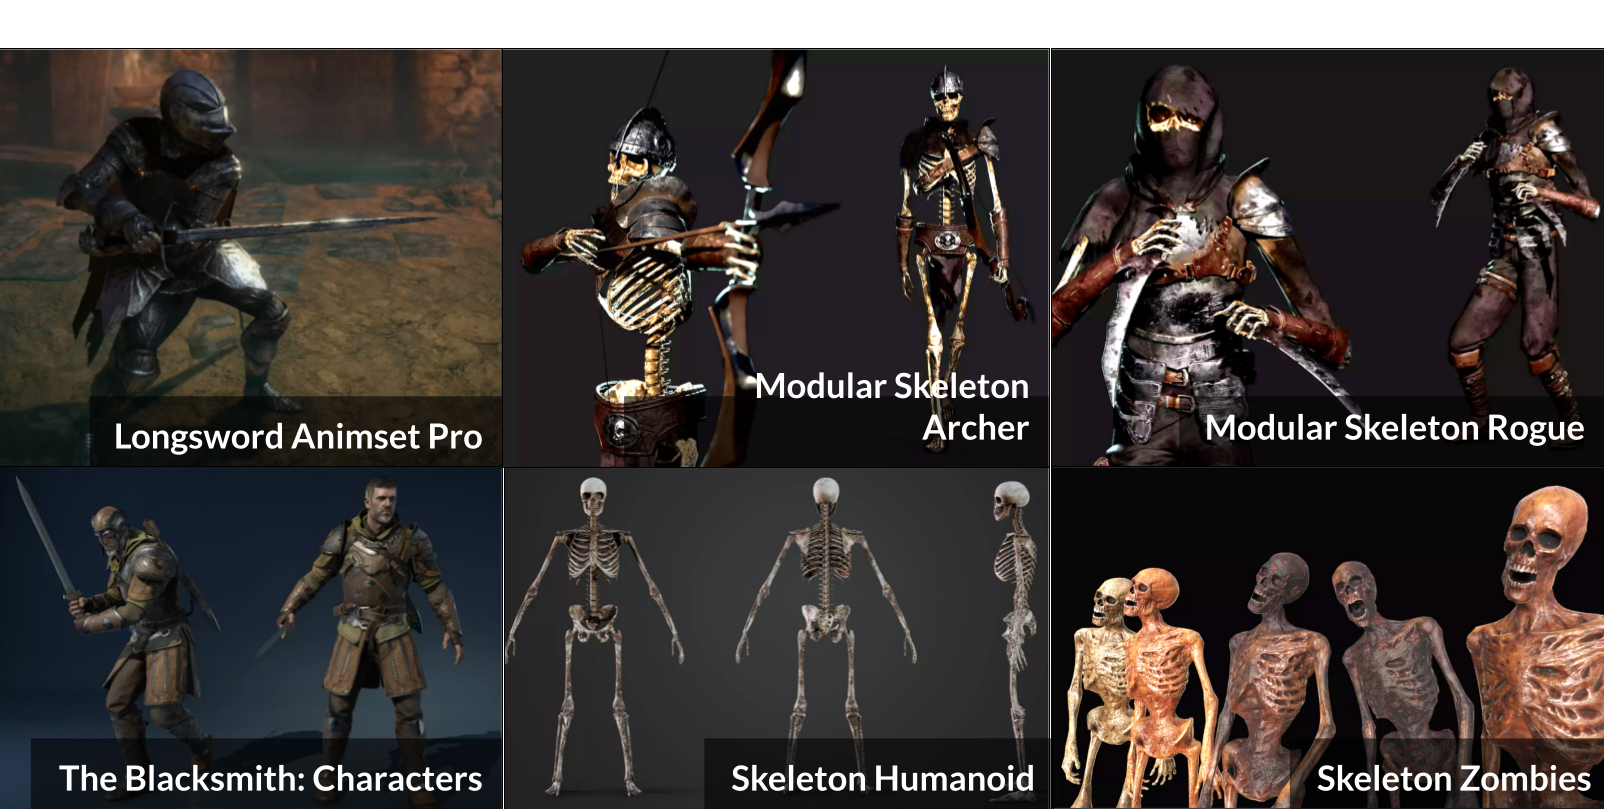
\includegraphics[width=30em]{figures/fig-character-assets.png}
        \legend{Source: Collation of screenshots performed by the authors from images captured from the original Unity Asset Store website pages for each of the assets used in this work.}
    \end{center}
    \label{fig:character-assets}
\end{figure}

% Talk about model for player Character: Blacksmith: Characters
When considering the options to represent the playable character, we must constrain our options to the aesthetic aspects of the Dark Fantasy genre, where a character would need to dress with the appropriate attire or armor pieces and should be able to wield common weapons from a Medieval thematic landscape such as swords and shields. The second criteria considers the gameplay aspects of our implementation, where we constrain the possible features to a definition of a standardized experience from the original game using the most popular equipment setup used by players -- the 'Sword and Shield' combination.

Therefore, we require a 3D model for a humanoid character that can be inserted in the context of a Dark Fantasy world, that can visually satisfy the \emph{Warrior} character archetype wielding a sword and shield, and that is compatible with the skeletal rig for an animation set that contains sword and shield animations. For this purpose, we selected the \emph{Challenger} character model from the \emph{Blacksmith: Characters} asset pack, which portrays a middle-aged warrior wielding a sword and shield and using leather body armor pieces. As with the 3D models selected for non-playable entities, the Challenger character is compatible with the \textsc{Mecanim} skeletal rig system from Unity, which provided compatibility with most animation asset packs from the \textsc{Unity Asset Store}.

% After that, we need animations that can be easily integrated with the designed combat system
To properly integrate the characters into the game world, and to provide visual feedback as to what actions characters are performing given their functional purpose in terms of gameplay aspects, we require animations for humanoid characters that are compatible with the \textsc{Mecanim} system and that are congruent with the purpose of each model. The animation set for each playable or non-playable character should appropriately reflect the weapons and other equipment that the character possesses, as well as the overall body proportions and weight of the attire being used.

An example of animations being congruent with the purpose of a character would be an archer enemy that has animations for wielding a bow, drawing arrows from a quiver and shooting arrows. Since the armor pieces for an archer enemy should be lighter in comparison to a heavy-armored warrior archetype enemy, the movement animations should include faster steps and less restricted joint rotations to reflect the weight of the light attire.

Considering these requirements, we selected the asset packs \emph{ZOMBIE Starter Animation Set}, \emph{Sword and Shield Animset Pro}, \emph{Longsword Animset Pro}, \emph{Archer Animset Pro} and \emph{Rogue Animset Pro}. Each of the animation sets selected for our implementation satisfies the functional requirements of roles designed for playable and non-playable characters, while also being compatible with the skeletal rig standard defined by the \textsc{Mecanim} system.

% Then, we need sound effects and ambient background music that mirror the affective purpose of sound in Dark Souls
We also require sound effects to provide a clear feedback of actions and consequences in the game world, such as a character moving, attacking, blocking an attack, getting hit by an attack or dying. The sound effects for our implementation were selected mainly because of their similarity to the sound effects of the equivalent effects in the original game. For instance, a sound effect for when a character is hit in the original game conveys both the weapon that is being used by the attacker and the scale of damage that is being applied to the target. A frontal attack presents less of a deep, impactful sound effect than a back-stab attack, which does a significantly higher amount of damage. For these reasons, we chose the asset packs \emph{Axe Swing \& Damage Sounds}, \emph{Medieval Fantasy 2 Audio} and \emph{Universal Sound FX} which contain a wide variety of sound effects representing medieval melee weapons such as swords, axes, shields and bows, while also providing a variety of impact levels for successful attacks.

For this project, the immersion of players in the environment of an abandoned castle was also considered, and thus we chose to add ambient background noises and music that could be looped for the duration of a session. As a base requirement for the selection of these noises, it was decided that they should provide a sense of depth to the scenery, with quieter sound effects for events that are closer to the player such as crumbling stone and crackling wood, and somewhat louder sound effects for events that are far away from the player, such as running water, fire and falling chunks of stone. As for the music, it should provide an overall sense of horror and mystery that goes in accordance with the Dark Fantasy genre. Therefore, we selected the asset packs \emph{Medieval Fantasy 2 Audio} and \emph{Dark Fantasy Audio} for ambient sound effects and music, which can appropriately convey the sense of an abandoned, crumbling castle while also containing music for an eerie environment.

% We also need Visual Effects that can go along with the sound effects to provide a proper visual feedback when the player hits an enemy. % 

In sequence, we require a collection of \emph{particle-based}\sepfootnote{fn:particle-vfx} visual effects to provide a proper visual feedback when characters are able to successfully attack their enemies, as well as visual effects that complement the aesthetics and purpose of the 3D models we selected for our environment. For conveying successful attacks, we chose to add pseudo-volumetric particles for a splatter of blood that originates from the body of the attacked target, with the asset pack \emph{Pseudo-Volume Blood Effects} being the most appropriate for this purpose. To increase the detail and depth of our 3D environment, we used fire particle effects for candle and small torches from \emph{Smoke \& Ember FX} and \emph{Unity Particle Pack}. In additional to fire particles, these asset packs also provided smoke particle effects, which were used to both complement the fire from light sources and to help occlude certain parts of our levels until the player moved to a closer position.

% We need 2D UI Elements that can convey the basic gameplay resources: Health and Stamina
We also need a collection of 2D UI Elements that are able to convey the basic gameplay resources that the player should be able to keep track of during a gameplay session: \emph{Health} and \emph{Stamina}. For this purpose, \emph{Health Bars} will suffice as they are a common standard for representing attributes that have a variable maximum value and a minimum value of zero. The design and layout of these elements should be in overall accordance with the Dark Fantasy genre, avoiding overly saturated color pallettes and an exaggerated geometric complexity.

% We also need UI Elements for menus, settings, tooltips and button captions
We also require a variety of UI elements that can be used for assembling the menus that will be used by the player to initiate sessions, pages for the configuration of game settings, small tooltips that provide a brief description of the functionality of UI elements, and button captions that can be displayed during a game session to provide the player with a reference of the actions that can be performed at any given time.

To represent most of the UI elements in our implementation, we selected the asset pack \emph{RPG \& MMO UI 5} which contains the most common UI elements used in the video games such as menus, buttons, tooltips, Health bars, loading screens and portraits, with an overall design tailored for Fantasy games. This asset pack also contains an under-saturated color palette with greyed out colors, which goes in accordance with our aesthetic needs for a Dark Fantasy game. For button captions, we selected the asset pack \emph{PC \& Consoles Buttons Icons} which contains button icons for a multitude of input devices such as Xbox Controllers, PlayStation Controllers, Mouse \& Keyboard and even joysticks for Head-Mounted devices.

% Finally, we used complementary editor tools that allowed for a more concise and streamlined workflow for serializing game data and implementing common functionality for third-person hack and slash games
We also included \emph{Odin Inspector} as a complementary editor tool that allowed for a more concise workflow when serializing game data such as character attributes, physics properties and gameplay values into binary game asset files. With \emph{Odin Inspector}, it was possible to create reusable serializable classes that could be assigned to components directly from the \textsc{Unity} engine editor, which was used as a base for the creation of our \emph{Attributes}, \emph{State Machines} and \emph{Performance Tracking} systems.

% Table showing Asset Name, Type, Size, Price, Path in Project
In conclusion, we use table \ref{tab:table-game-assets} to provide a consolidated list of the assets discussed in this section, along with the appropriate extraction paths for the assets to work with our source code.

% Table: List of game assets
\begin{table}[!h]
    \begin{center}
      \caption{A consolidated list of the assets used in the implementation of this work.}
      \label{tab:table-game-assets}
      \rowcolors{2}{}{gray!25} % Alternate row colors
      \begin{tabular}{ >{\small}w{l}{11em} >{\small}w{c}{4em} >{\small}w{c}{3em} m{13em} } % alignments and column size
        \addlinespace
        \toprule
        % Headings
        \textbf{Name}                & \bf Type  & \bf MSRP & \textbf{\small Path in Project}                             \\
        \midrule
        % 3D Models
        Fantasy Dungeon              & 3D Models &  \$90.00 & \texttt{\tiny Assets/AssetStore/3D/FantasyDungeon/}      \\ 
        Skeleton Zombies             & 3D Models &  \$16.00 & \texttt{\tiny Assets/AssetStore/3D/StudioNewPunch/}      \\
        Modular Skeleton Archer      & 3D Models &  \$34.99 & \texttt{\tiny Assets/AssetStore/3D/SkeletonArcher/}      \\
        Modular Skeleton Rogue       & 3D Models &  \$34.99 & \texttt{\tiny Assets/AssetStore/3D/SkeletonRogue/}       \\
        Skeleton Humanoid            & 3D Models &  \$19.99 & \texttt{\tiny Assets/AssetStore/3D/SkeletonHumanoid/}    \\
        The Blacksmith: Characters   & 3D Models &     FREE & \texttt{\tiny Assets/AssetStore/3D/ChallengerCharacter/} \\
        \midrule
        % Animations
        ZOMBIE Starter Animation     & Animation &   \$4.99 & \texttt{\tiny Assets/AssetStore/3D/ZombieAnimset/}       \\
        Sword and Shield Animset Pro & Animation &  \$65.00 & \texttt{\tiny Assets/AssetStore/3D/SwordShieldAnimset/}  \\
        Longsword Animset Pro        & Animation &  \$50.00 & \texttt{\tiny Assets/AssetStore/3D/LongswordAnimset/}    \\
        Archer Animset Pro           & Animation &  \$55.00 & \texttt{\tiny Assets/AssetStore/3D/ArcherAnimset/}       \\
        Rogue Animset Pro            & Animation &  \$50.00 & \texttt{\tiny Assets/AssetStore/3D/RogueAnimset/}        \\
        \midrule
        % Sound effects and Music
        Axe Swing \& Damage Sounds   & SFX       &   \$5.00 & \texttt{\tiny Assets/AssetStore/Audio/AxeSwingSounds/}   \\
        Medieval Fantasy 2 Audio     & SFX       &  \$50.00 & \texttt{\tiny Assets/AssetStore/Audio/MedievalFantasy2/} \\ 
        Universal Sound FX           & SFX       &  \$40.00 & \texttt{\tiny Assets/AssetStore/Audio/UniversalSoundFX/} \\
        \midrule
        % Music
        Dark Fantasy Audio           & Music     &  \$22.99 & \texttt{\tiny Assets/AssetStore/Audio/DarkFantasyAudio/} \\
        \midrule
        % Visual Effects
        Pseudo-Volume Blood Effects  & VFX       &  \$15.00 & \texttt{\tiny Assets/AssetStore/VFX/KriptoFX/BloodFX/}   \\ 
        Smoke \& Ember FX            & VFX       &  \$10.00 & \texttt{\tiny Assets/AssetStore/VFX/SmokeEmberFX/}       \\ 
        Unity Particle Pack          & VFX       &     FREE & \texttt{\tiny Assets/AssetStore/VFX/UnityParticlePack/}  \\
        \midrule
        % UI Elements
        PC \& Consoles Buttons Icons & UI        &  \$14.99 & \texttt{\tiny Assets/AssetStore/UI/PCConsolesIcons/}     \\ 
        RPG \& MMO UI 5              & UI        &  \$35.00 & \texttt{\tiny Assets/AssetStore/UI/RPGMMOUI5/}           \\
        \midrule
        % Editor Utilities and Extensions
        Odin Inspector               & Plugin    &  \$55.00 & \texttt{\tiny Assets/Plugins/Sirenix/}                   \\ 
        \bottomrule
      \end{tabular}
    \end{center}
  \end{table}

% ============================================================================
% ============================================================================
% ============================================================================

\section{Gameplay Mechanics and Systems}

% Overview of all gameplay subsystems
% - Here we talk about the subsystems that involve the player-controlled character in our implementation and how it interacts with non-playable entities
% - Figure: Player components and class diagram
% - Movement mechanics with collision handling for walls and obstacles, detection of slope thresholds and handling of gravity and fall damage
% - A character animation systems that reacts to actions performed by the player and any events that might affect the status of the player, such as hits taken, staggering and death
% - A third person camera that allows the player to orbit the viewport around the game character, while also constraining its position and viewport contents to the boundaries of a playable environment
% - A lock-on camera that is able to frame the player and a target enemy character, and which is coupled with a target prioritization system for enemy characters, and that allows the player to switch targets
% - A combat system which handles hit and block detection, combat effects such as stamina draining, damage and poise break, attack action and state handling, and combat statuses that affect the ability of a character performing actions
% - An attributes system that can be containerized into components for game entities, is able to serialize value data types, broadcasts events when its values are changed, and can be used by other gameplay subsystems to determine the status of a game entity
% - A character status system that accounts for Invincibility Frames (IFrames) when dodging and the inability of performing actions when staggered or dead

% ============================================================================
% ============================================================================
% ============================================================================

% Movement mechanics and physics
\subsection{Movement mechanics and physics}

% - CharacterController for wall and obstacle collision and running over slopes

Traditionally, the movement for player-controlled characters in games is not made to be physically realistic. Characters will often move at abnormally high speeds, are able to stop almost immediately and can turn their movement direction with ease. This is made so that character movement is highly responsive to player input and becomes easier to manipulate in comparison to physics-based controls. If player characters in video games were to be physically accurate, they would take significant time to accelerate to their maximum movement speed and decelerate until stopped, while also having difficulty turning sharp angles at high speeds.

For gameplay purposes, characters implemented with physical accuracy feel heavy and difficult to control, forcing the player to consider  physical properties of their characters and the geometry of the environment. This causes a significant amount of overhead for the player to obtain proficiency with motion controls. In general, character movement should be a streamlined, trivial mechanic that can be quickly learned by the player. Learning motion controls in a game should not get in the way of the player partaking into the core gameplay loop\sepfootnote{fn:core-gameplay-loop}, unless movement in itself is part of the core game loop as in \emph{Death Stranding}\sepfootnote{fn:death-stranding}.

Considering the need for responsive movement that can be easily mastered, we use the implementation of a \emph{CharacterController}\sepfootnote{fn:character-controller} component that is natively built-in as part of \textsc{Unity}'s base functionality. CharacterControllers are not affected by Unity's physics system, are able to slide along walls when moving against them over a non-orthogonal angle, to detect and move over small vertical offsets in ground geometry such as steps and ledges, and to handle movement in slopes.

The movement input from a player will generate different motion types depending on camera state. In the default state of a Third-Person Orbital Camera, movement input will cause the player character's body to rotate to face a direction relative to the camera's viewport, while also causing the body to move forward according to its current rotation. The Movement System broadcasts the signal that the player is always moving forward, which is received and handled by the Animation System. In this camera state, motion itself is handled by the animations so that the movement speed perfectly matches the animation being played and avoiding \emph{movement drifting}\sepfootnote{fn:movement-drifting} issues.

While this setup of the Movement System handling body rotation and the Animation System handling motion itself does cause the player to move in the direction defined by their input, this also requires a \emph{maximum rotation speed} to be taken into consideration. A character should be unable to immediately turn to the opposing movement direction, with the \emph{maximum rotation speed} constraining the speed at which a player is able to turn.

In the state where the player performs a \emph{Lock-On}\sepfootnote{fn:lock-on} targeting an enemy character, movement input causes the player to directly move at a direction without changing its body rotation. In this state, body rotation is handled by the camera system, where the player-controlled character will always face an assigned target. The Animation System will use movement input to blend between multiple movement animations such as forward movement, side steps and back steps. Movement motion in this state is still relative to viewport direction, but the viewport in itself is positioned relative to the player and their target. Camera positioning for \emph{Locked-On Cameras} will be further explained in subsection \ref{sec:lock-on-camera}.

Another state that should be considered for motion controls is when the player is not touching the ground. In technical terms, the Capsule-shaped \emph{collider}\sepfootnote{fn:colliders} from the player CharacterController would not \emph{overlap}\sepfootnote{fn:collider-overlapping} with ground geometry. In this situation the player character should be considered "On-Air", and movement input should have less of an influence in motion and body rotation or no influence at all, as being able to accelerate, decelerate and quickly turn without ground friction would be considered implausible by players and could possibly break immersion. When the player is not on ground, we constantly accelerate our CharacterController velocity by a gravity vector on fixed time steps defined by the \emph{FixedUpdate}\sepfootnote{fn:fixed-update} event of the \emph{MonoBehaviour}\sepfootnote{fn:monobehaviour}.

% - Gravity and grounded state detection

To detect if a player is ground or not, we make use of \emph{Unity's} built-in \emph{SphereCast} operation, which iterates performing multiple overlaps of a sphere with a radius slightly higher than the radius of our CharacterController with the ground geometry, along a direction defined by a \emph{Ray}\sepfootnote{fn:rays}. The ray originates from the center of the body of the player-controlled character, and extends along the direction of the gravity vector in a length of three quarters of the vertical size of the CharacterController capsule collider. This is done so that vertical collisions can be detected ahead of time when the player is falling at high speeds, avoiding the common problem in video game physics where the player becomes stuck inside ground geometry.

\begin{lstlisting}[caption={Implementation of grounded state detection.},label={lst:grounded-detection}]
var ray = new Ray(transform.position, Vector3.down);
grounded = Physics.SphereCast(ray, charController.radius + 0.1f, charController.height / 2f + 0.5f, physicsData.GroundDetectionLayers.value);
// Animator also applies gravity, so when not grounded disable animator physics
player.Anim.applyRootMotion = grounded;
\end{lstlisting}

An advantage of using \emph{Raycast-type}\sepfootnote{fn:raycasts} operations instead of frame-by-frame collision overlap detections is that Raycasts are able to precisely detect the points where a collider starts overlapping with the ray along a fixed length of an axis. This enables us to pinpoint which parts of our collider the ground geometry touches and the exact moment the ground geometry first makes contact with our character, being the optimal operation to use when considering objects that are moving along an axis over time -- which is the case for the player being affected by gravity in our implementation.

In contrast to using a regular Raycast, the SphereCast operation is able to detect overlaps in a volume, which means that complex collider setups which overlap in the borders of our CharacterController will still be detected. A common situation in games where platforms and gravity can affect the player is that players might find themselves over one or multiple ledges, where a single Raycast operation would not be able to handle colliders that are in the edges of a CharacterController.

% Figure: Example showing visual difference of Raycast vs SphereCast

In games where grounded-state detection is not handled appropriately, Character controller components will often accumulate vertical velocity indefinitely, since while being impossible to move downwards due to the character controller constraining movement against colliders, the 'grounded' state is never detected. What commonly happens after this is that when the player steps away from the ledge sufficiently, they will instantly fall to the ground instantly because of the accumulated speed. If the game is programmed to apply fall damage in this situation, this might mean instant death even though the player did not fall from a considerable height.

Finally, in the frame where a character that was previously considered not groun\hyp{}ded detects ground collision, we invoke the \textsc{OnHitGround} event, and proceed to perform fall damage calculation. In our implementation, fall damage is calculated by considering fall speed multiplied by a parametrized speed-to-health-point conversion factor, named 'FallDamageMultiplier'.

Figure \ref{fig:movement-class-diagram} shows an overview of the class architecture for our implementation of the movement system. We have a top-level \textsc{Player} class which holds the components for all gameplay-related subsystems. The \textsc{PlayerMotor} component is an implementation of the \textsc{ICharacterMotor} abstraction, and is responsible for implementing the movement and physics logic of our motion controls.

When input is received from the user, the \textsc{PlayerMotor} component filters the input, calculates movement direction based on viewport orientation, and redirects the actual transform position changing to \textsc{Player.Move()}. The \textsc{Player} class in turn calls \textsc{CharacterController.Move()} that considers collisions and other physics-related constraints, and broadcasts movement signals that will be consumed by the \textsc{PlayerBody} class, which is responsible for handling character animation.

% Figure: Player Movement Class Diagram for Bright Souls
\begin{figure}[!ht]
    \begin{center}
    \caption{Class diagram representing the architecture of our Movement System.}
    \vspace{0.5em}
        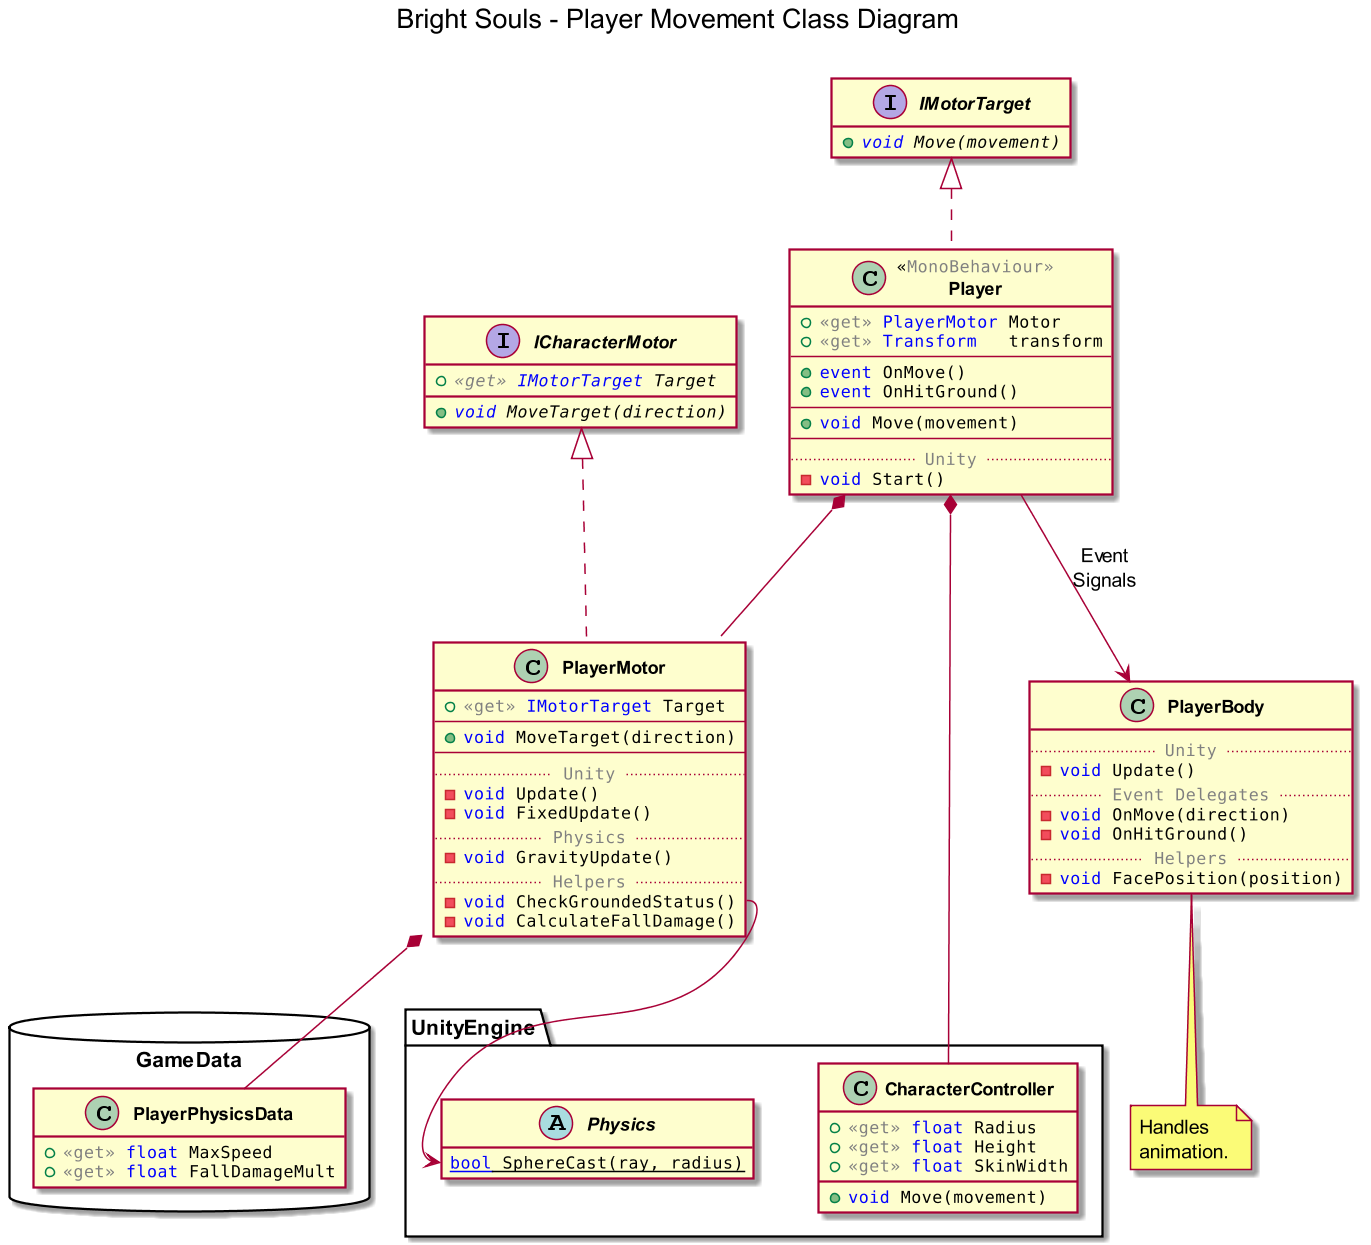
\includegraphics[width=34em]{figures/fig-player-movement-class-diagram.png}
        \legend{Source: Diagram assembled by authors.}
        \label{fig:movement-class-diagram}
    \end{center}
\end{figure}

% ============================================================================
% ============================================================================
% ============================================================================

\subsection{Camera System}
\label{sec:lock-on-camera}

% In this implementation, we design and implement two separate camera modes
%   - Orbital Third Person Camera
%       > Commonly used for third person hack n' slash or platforming games
In our implementation, we use our analysis of \emph{Dark Souls} in section \ref{sec:analysis-dark-souls} to design two separate camera modes with complementary functionality that can be used as tools for the player to achieve optimal performance in and out of combat. First we implement an \emph{Orbital Third Person Camera}, which is commonly used in third person \emph{Hack and Slash} and \emph{Platforming} games where the player has to evaluate the properties of the environment they are in and quickly assess dangers that might cause their defeat to devise a plan of action.

%       > Camera positions itself in the perimeter of an ellipsoid that is centered on the player
%       > Input from the player generates movement along the perimeter, causing the camera to orbit around the player
%       > Attempts to frame both the player and the environment by using a position above the player as pivot
An Orbital Third Person Camera positions itself in the perimeter of a three dimensional ellipsoid that is centered on the player, where input from the player generates movement along this perimeter. This type of camera attempts to frame both the player and the environment at the same time, having the player on a central position in the screen and using a position above the player as a rotation pivot. The rotations from player input along with the framing algorithm causes the camera to perform an orbital movement.

%       > In our game, it is the default camera mode, used for traversal around the map
%       > Free control over framing enables player to scout for enemies, avoid pitfalls
In our game, Orbital Third Person Cameras are the default camera mode, and are mainly designed for traversal around the three-dimensional environment. The fact that the player has control over the positioning and framing of the camera enables the player with the possibility to scout the environment for pitfalls and enemies before performing movement. This is the perfect type of camera to be used in out-of-combat situations in third person games, as players can gather information safely and use it to devise a plan-of-action.

%   - Lock-On camera
%       > Mostly used in action third person hack n' slash games that have melee combat, although some RPGs also use it
%       > Camera positions itself behind the player and attempts to frame both the player and a target character
The second type of camera in our implementation is the \emph{Lock-On Camera}, which is mostly used in action third-person \emph{Hack and Slash} games that have melee combat. This type of camera positions itself behind the player character, and attempts to frame both the player and a target -- most commonly an enemy character. Whenever the target character moves, the camera adjusts its position and framing to maintain a fixed relative positioning between the player character and their target.

%       > Camera positioning and framing creates fixed "dimensions of movement" of the player relative to a target,
%         making it easier for a player to avoid attacks from that target and find the optimal spacing to land their
%         own attacks
The relative positioning and framing of a Lock-On Camera creates fixed axes of movement between the player character and their target where if a player moves horizontally, they will move in a circle around the target character. Moving forward and backwards adjusts the distance between the player and their target. The purpose of this mechanism is for the player to have better control of spacing during combat, making it easier for the player to avoid attacks and find the optimal distance to land their own attacks.

%       > Useful for the player to be able to track and attack a single target with ease without missing,
%         instead of having to specify a "direction" for the attack, the player can simply press the attack button
%         and the character will already be facing the enemy and perform the attack in the correct direction
The fact that a Lock-On Camera is always facing a single target character removes the necessity for players to specify a direction for their attacks through input. Instead, players can simply press the attack button when their characters are within attack range. Since the character is constantly facing the enemy, the direction of their attack is guaranteed to be correct. Another positive effect caused by this behavior is that the framing helps the player to focus on the actions being performed by the enemy character, helping to understand when an enemy is attacking and which kind of attack an enemy is performing.

%       > Has issues in environments in constrained spaces, where the enemy is too close to the player or the player
%         is too close to a wall. Framing becomes an issue in this case
However, Lock-On camera implementations face issues when the target character is too close to the player character, or when they are operating in environments with constrained space. When the player character is too close to their target, it is common for Lock-On cameras to not adjust their vertical offset, meaning that the framing direction must be angled downwards and into the ground. This causes the player to have limited geometric information about the surroundings of both characters, making it harder to efficiently navigate the environment during combat. Furthermore, if a player is moving horizontally when close to their target, the perimeter of the circle of movement has a significantly reduced radius, making the camera rotate at high speeds and causing motion sickness\sepfootnote{fn:motion-sickness} in some instances.

When Lock-On cameras operate in constrained space, it is common for the default offset position to be located outside the playable space (e.g. inside walls), and thus a position resolution algorithm is required to guarantee that the camera is always in a valid position. The most common algorithm is the pull-forward approach, where if the camera would be located outside the playable space the target position is recalculated so that the camera is brought closer to the player. While this solution works until a certain point, if the player positions their character too close to a wall it might create a situation where it is impossible for the camera to frame both the player and their target, with either the player character occluding the target or the camera focusing solely on the target by being positioned above the player character. In addition, a similar problem to that of players being to close to targets occurs, where in this case the camera might reposition too quickly due to the resolution algorithm.

Figure \ref{fig:camera-types} shows a comparative diagram of both camera types implemented in this work, where four screen captures are used for the Orbital Third Person Camera to illustrate multiple framing angles that can be achieved from player controlled rotations.

% * Figure: Orbital and Lock-On camera framing/rotation
\begin{figure}[!ht]
    \caption{Comparative screenshots showing the difference between the Orbital and Lock-On camera modes.}
    \vspace{0.5em}
    \begin{center}
        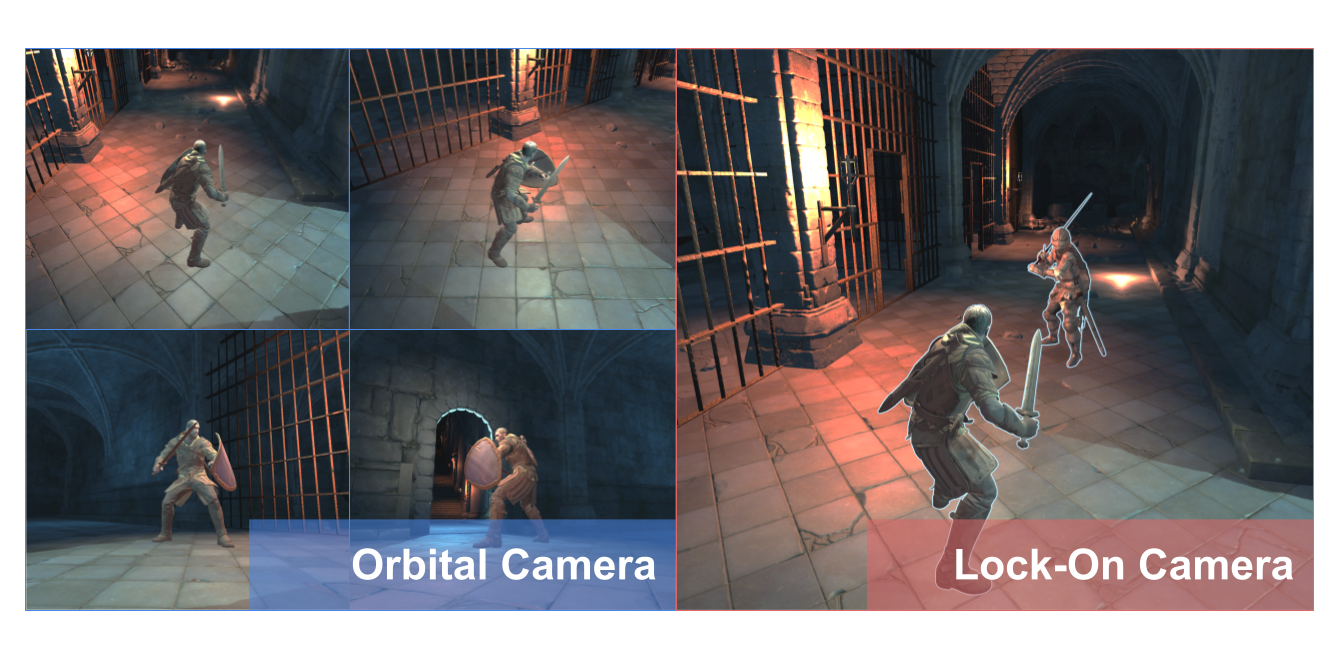
\includegraphics[width=34em]{figures/fig-camera-types.png}
    \end{center}
    \legend{Source: Screen capture of application developed by authors.}
    \label{fig:camera-types}
\end{figure}

% Third Person Orbital Camera implementation
% - Use of Cinemachine
%     - Ready-to use implementation of orbital rotation with parametric spline curve for vertical axis
%     - Smooth transition between virtual cameras which was useful for Orbital Camera and Lock-on modes
Regarding the implementation of the Orbital Camera, we chose to use the \emph{Cinemachine} Unity Package due to its comprehensive API and functionality for multiple types of cameras, including specific algorithms to manipulate Orbital Cameras. Another useful trait is that the APIs provided by Cinemachine enable defining parametric curves for positioning, which increases the expressive power of game designers.

%     - Algorithmic motion that can simulate cinematic behavior with camera shake effect and framing corrections
Cinemachine can also manage, compose and blend multiple cameras, which is useful to perform shot transitions triggered by a signal system that resembles the \emph{Observer} pattern\sepfootnote{fn:observer-pattern}. Cinemachine also includes algorithms for procedural motion generation, which is used to create screen shake effects with high fidelity when the player is attacked by an enemy, or to properly adjust framing when the camera needs to track movement of high velocity targets.

% Prefab GameObject hierarchy with CinemachineBrain at root 
% MainCamera object as a child of the CinemachineBrain
We start by creating a \textsc{Prefab}\sepfootnote{fn:unity-prefabs} hierarchy of \textsc{GameObjects}\sepfootnote{fn:unity-gameobjects} where we include a \textsc{CinemachineBrain} component in the root level, and multiple \textsc{VirtualCameras} as child objects. The \textsc{CinemachineBrain} component is responsible for defining the current active camera, camera transitions and the signals that trigger each transition. The \textsc{CinemachineBrain} brain component requires a reference to a \emph{Main Camera}, a special \textsc{GameObject} with a \textsc{Camera} component responsible for rendering the final output of our camera management system. We add the \emph{MainCamera} object as a child of the root.

% VirtualCamera child objects that contain definitions for transposing and composing strategies
As child GameObjects of the hierarchy root, we include a set of \textsc{VirtualCameras} for each of the camera modes in our implementation. In this case, we simply add a VirtualCamera for the Orbital Camera and another for the Lock-On Camera. VirtualCameras are Cinemachine abstractions that define the physical properties of a camera along with transposing and composing strategies\sepfootnote{fn:transposing-and-composing}. In this case, we use a VirtualCamera with an Orbital transposing strategy and a single LookAt target aiming at a pivot position above the player character. For the Lock-On camera, we use a simple Follow strategy for transposing and a Group Composition strategy to frame both the player character and their target enemy.

% PlayerCameraDirector component, which is responsible for receiving signals from player and translating them into signals for the CinemachineBrain and activating and deactivating PlayerCameraBehaviours
We also add a \textsc{GameObject} containing a \textsc{PlayerCameraDirector} component, which is responsible for receiving signals from the \emph{Player} component and translating them into signals for the \textsc{CinemachineBrain}. The signals are then used to switch and transition between shots. The \textsc{PlayerCameraDirector} is also responsible for enabling and disabling \textsc{PlayerCameraBehaviour} components, which receive player input, manage camera framing targets and initialize camera states.

The \textsc{VirtualCamera} components are tasked with receiving player input and performing the appropriate actions given the input. For instance, the \textsc{OrbitalCamera} receives a two-dimensional vector as input, which is translated into vertical rotation and translation for the Y axis and horizontal for the X axis. In the Lock-On camera, the horizontal axis of the vector input is used to switch Lock-On targets. Figure \ref{fig:camera-class-diagram} shows an overview of the class relationship in our camera system implementation, as well as the signals that are being sent and listened to.

% * Figure:  Camera system class diagram
\begin{figure}[!ht]
    \begin{center}
    \caption{A diagram showing the class relationship of our Camera System implementation, along with the signals being sent and processed.}
    \vspace{0.5em}
        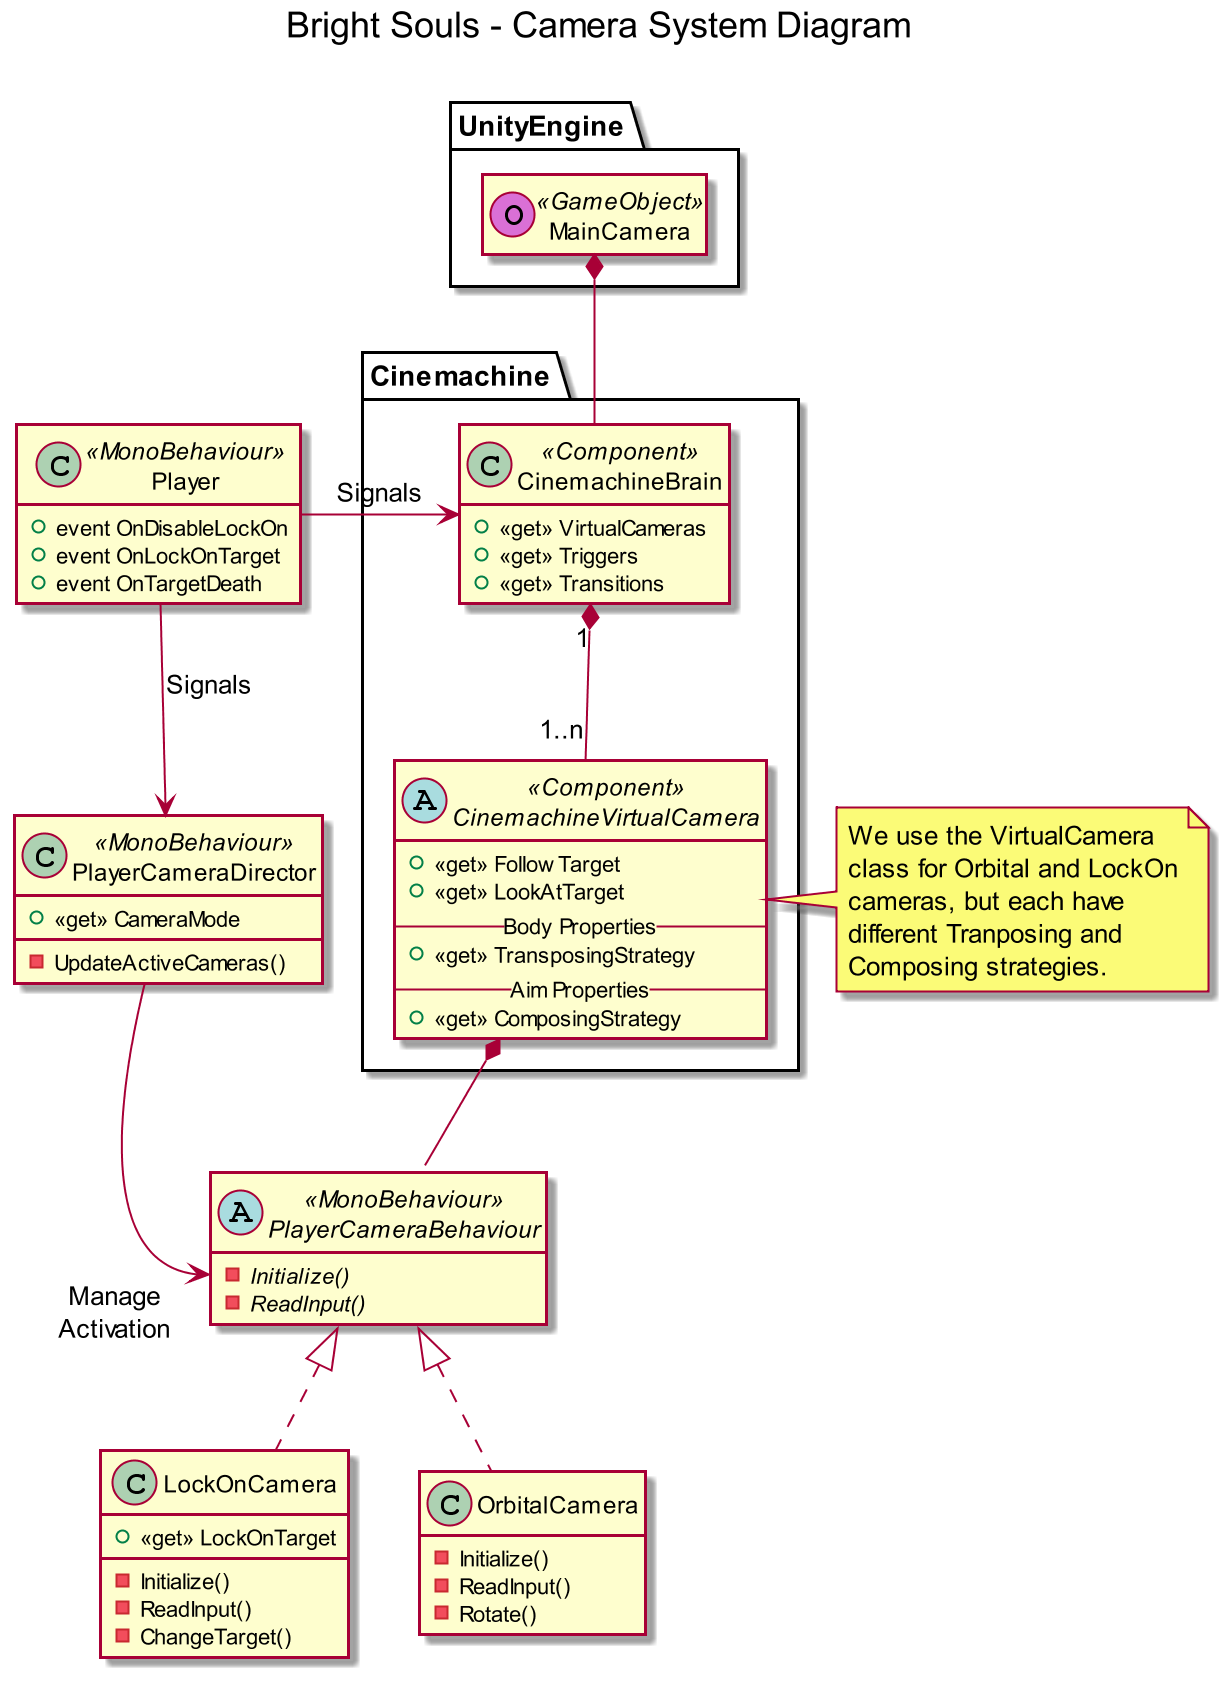
\includegraphics[width=34em]{figures/fig-camera-system-class-diagram.png}
        \legend{Source: Diagram assembled by the authors.}
        \label{fig:camera-class-diagram}
    \end{center}
\end{figure}

%     - Simplified collision geometry enables using a pull-forward collision resolution
For position resolution, we created a simplified and invisible collision map to define the constraints of where a camera can be positioned in a game level. This is done to both improve the performance of raycasts and to avoid jittery movement when using pull-forward collision resolution on thin objects. This collision map is limited to interact with camera algorithms, and does not affect player movement or any other physics entities in any way.

% Lock-On camera and targeting system
% - Possible Lock-on targets must be located in an intersection of the camera viewport with a collision sphere centered at player character
% - Lock-On target prioritization is higher for targets that are closer to the player and to the center of the screen
To detect Lock-On eligible targets, we use a spheric collider in a radius around the player collider and intersect any detected entities with those present in the viewport, to constrain selection to entities being visualized. Eligible targets are collected into a list ordered by distance to the player character, which is updated every second. This is done because targets that are closer to the player are considered a higher threat, as they are more likely to hit the player when attacking.

% - Use of horizontal input axis from Orbital Camera to switch between targets
Horizontal input from the player is used to switch between targets, where moving the input axis to the left switch to the closest target at the left of the current Locked-On target, using coordinates relative to viewport space. Therefore, the position of the next target is selected using a comparison of the position of the entity in the X-axis when converting their coordinates to a viewport space.

% ============================================================================
% ============================================================================
% ============================================================================

\subsection{Attributes System}

% Attributes system
Attributes are our abstraction for runtime data that represents the current state of a gameplay entity, such as the Player Character, an Enemy Character or even an interactable object in a level such as a door. Attributes can be initialized, serialized and monitored by external components and are used by a multitude of gameplay related systems. In our implementation, attributes are mostly used to represent combat related variables such as Health, Stamina and Poise, and thus are affected by events triggered by the combat system, such as Stamina being used when the player attempts to attack an enemy, or the Health lost when an enemy succesfully hits the player.

% Based on Generics: Attributes can be generated for any primitive type, such as int, float, double, string.
%   - Serialized into binary gameplay data files for game designers to define the default and maximum values for character health, stamina and poise
%   - Initialized by persistent data managers to maintain player status when transitioning between levels
Attributes are based on \textsc{C\#} \emph{Generics}, and can be generated for any value type such as integers, floating point variables, strings and enumerations. This limitation is imposed in our architecture so that attributes can be easily serialized into binary data files that can be used to define the default and maximum values for each attribute holder. This constraint also facilitates Attribute initialization, which is useful to support persistent data such as maintaining attributes between levels  or loading the state of an entity from a file in a savegame system. 

%   - Monitored by UI systems to display relevant data about the status of the player, for instance a Health Bar that display the current health of the player and shows health lost when getting attacked.
All Attribute types implement the \textsc{IAttribute} interface, which exposes acessors for data manipulation and events for value changes. This facilitates the use of attributes by separate, independent systems in our architecture. For instance, Attributes are monitored by UI (User Interface) systems to display relevant data about gameplay entities, such as the status of the player. Health bars show the current player health and also provide a good estimation of health lost when getting attacked by an enemy using a secondary, trailing health bar.

The advantage of creating of an event monitoring system between Attributes external systems is that upon initial conception of the architecture, we do not exactly know how many components will require communication with each gameplay entity. For instance, when implementing the UI for the player character we can initially propose a single health bar that would simply read the value of runtime variables from the \textsc{Player} class, but if we iteratively add new elements such as floating text, combat messages and visual effects, each of these systems should have direct access to the components that hold data regarding player state, which enforces component coupling in our architecture. With an event system, we can simply subscribe to signals being sent by attributes, constraining the exposed data and methods and facilitating component decoupling.

% - AttributesContainers
%     - Containerization of attributes to allow for entities with different attribute configurations without defining static types
%     - Possibility to dynamically assign attributes during the course of a session, which can be useful for a telemetry system
% - Definition of interfaces that expose attributes to any of the classes that might require it
Attribute owners will often contain different sets of attributes to satisfy the requirements of the systems they interact with. As such, characters that can partake into combat encounters will present different attributes in relation to interactable objects such as doors. To provide a standardized interface for the access of attributes over different entity types, we containerize attributes into \emph{Attribute Containers}, which provide a public interface for dynamic access and manipulation of statically typed attributes contained within an entity. Figure \ref{fig:attributes-diagram} shows an overview of the class relationships in the Attributes System, along with examples of how attributes signalize changes to external components such as UI Elements.

% * Figure: Attributes system class diagram
\begin{figure}[!ht]
    \begin{center}
    \caption{Class diagram for the Attributes System, showing examples of signals being used by UI Elements.}
    \vspace{0.5em}
        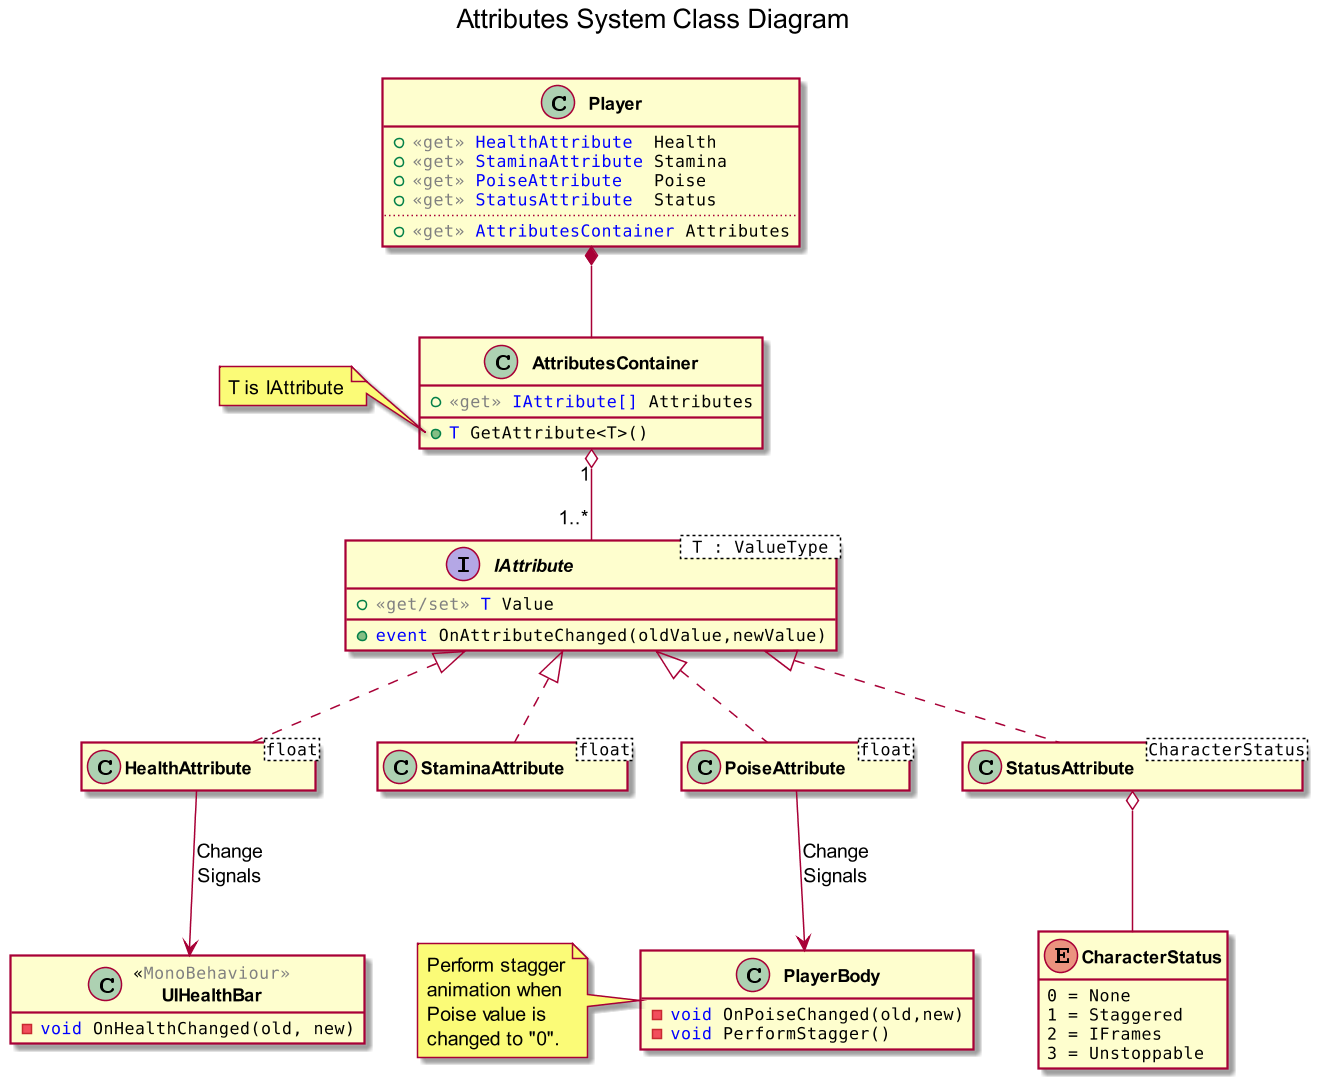
\includegraphics[width=34em]{figures/fig-attributes-diagram.png}
        \legend{Source: Diagram assembled by the authors.}
        \label{fig:attributes-diagram}
    \end{center}
\end{figure}

% ============================================================================
% ============================================================================
% ============================================================================

\subsection{Combat System}

% Combat System involves:
% - Managing attacking and combo animation and logical states for the player
% - Being able to detect when the weapon of the attacker collides with a target
% - Being able to detect when the target was able to block or dodge an attack
% - Applying combat effects when the target is hit
To implement combat mechanics in a \emph{Souls-like} game, we need a set of functionality components that are able to:
\begin{itemize}
    \item{Manage attack animations and logical states for the player character;}
    \item{A \emph{Hit Detection System} which is able to detect when the weapon of the attacker overlaps with the \emph{Hitbox} of a target to validate a \emph{Succesful Hit};}
    \item{Verify if attacks are blocked or dodged, and apply modifiers to Combat Effects;}
    \item{Apply \emph{Combat Effects} when a target is hit, such as a \emph{Health Damage} effect;}
    \item{Modify character state according to the effects that are applied.}
\end{itemize}
By combining the functionality aforementioned with AI agents that also make use of the same components, we can create a credible Combat System that provides appropriate feedback to player actions and decisions. In figure \ref{fig:combat-system-overview}, we provide an overview of the subsystems and classes regarding to our implementation of a Combat System.

% * Figure: Combat System Overview Diagram
\begin{figure}[!ht]
    \begin{center}
    \caption{A class diagram containing an overview of the class relationships in our Combat System implementation.}
    \vspace{0.5em}
        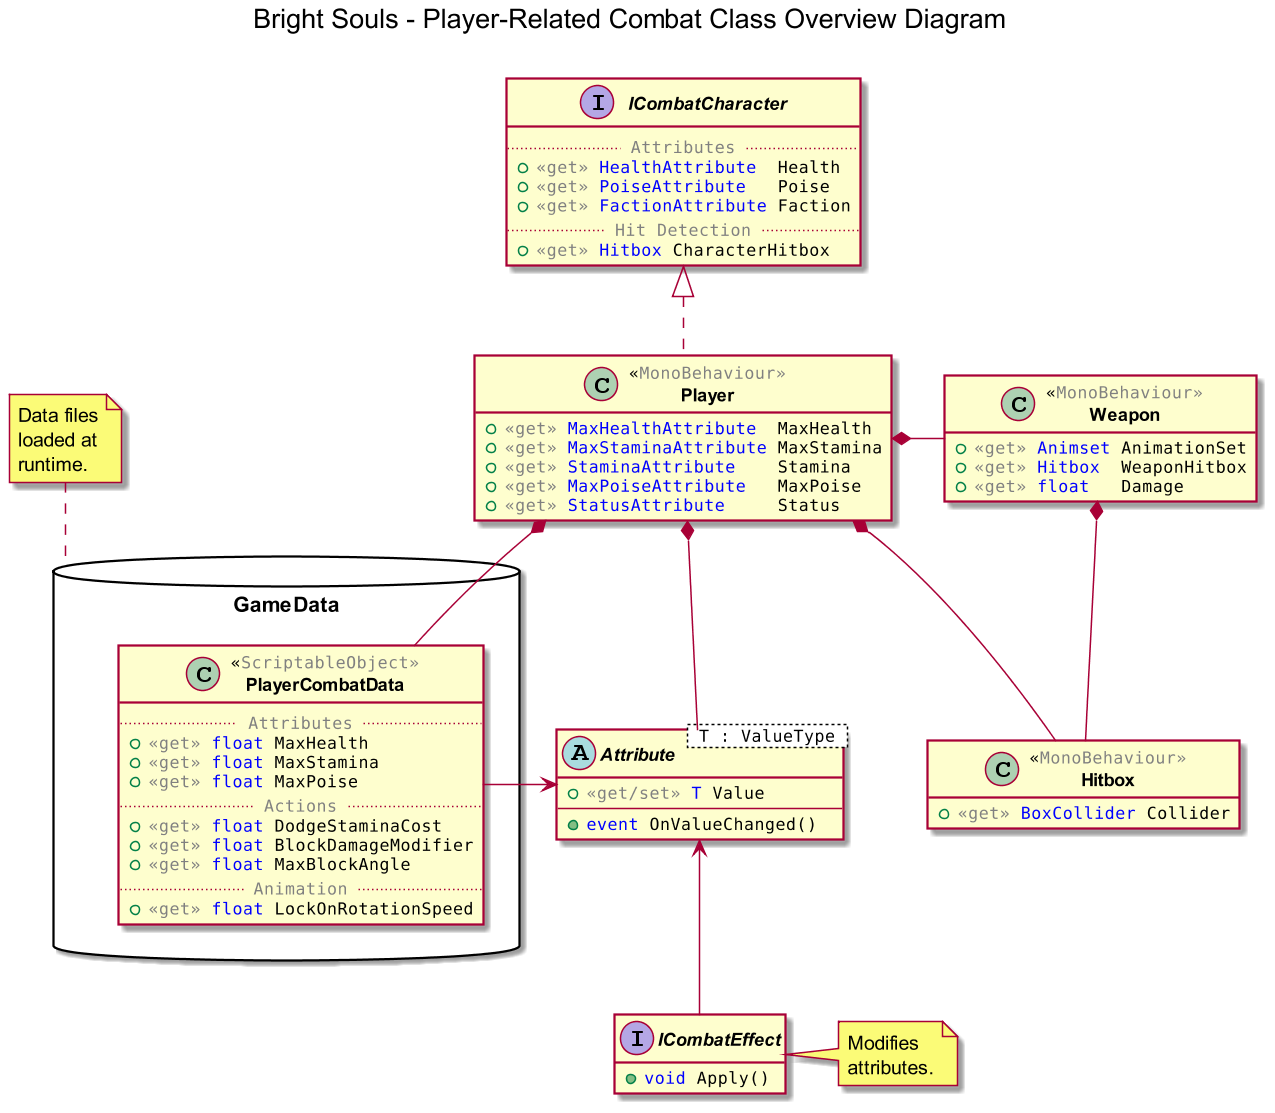
\includegraphics[width=34em]{figures/fig-combat-system-overview.png}
        \legend{Source: Diagram assembled by authors.}
    \end{center}
    \label{fig:combat-system-overview}
\end{figure}

% Attacking and combo system
%  - Continuously check for Attack input
We begin by listening to input from the player to determine when an \emph{Attack Command} should be issued. If the button mapped to the \emph{Attack Command} is pressed, we proceed to verify the current state of the player character to determine if an attack can be performed. The current state of the player is defined by a composition of boolean variables that reflect by the Animation being played on their character model.

% - Player/character is unable to perform attack if on Animation Lock
% - Attacks cost Stamina
If the character model is in the \emph{Dead}, \emph{Staggered}, \emph{AttackEnding}, \emph{On-Air}, \emph{Landing}, \emph{Dodging} or \emph{Blocking} animation states, the player is unable to perform an attack. This is commonly referred as \emph{Animation Locking} in games, and is an important aspect to potentially punish the player when taking strategically negative decisions. Attack Commands also have a resource cost for the player, where each attack depletes an amount of \emph{Stamina}. If the player Stamina resource has a value of zero, the player is unable to perform an attack. If the player has any Stamina value above zero, they are able to perform the attack.

%  - When sending attack command, enter a "combo" state and "Attack animation state machine"
%  - "OnCombo" state:
%    - Preemptively read player input before current attack animation ends. If player successfully sent attack input, continue the combo.
%    - If no attack input command is read within animation time frame, escape the Attack animation state machine
After an Attack Command is successfully validated, player state is set to \emph{Attacking} and the player enters an \emph{Attack State Machine} where Attack Commands are preemptively verified during attack animations. If an Attack Command is successfully executed before an attack animation ends an \emph{Attack Chain} is toggled, meaning that another attack animation is queued and transitioned to when the current attack animation ends. This behavior is commonly referred to as a \emph{Combo} in video games. Figure \ref{fig:player-anim-state-machine} shows the state machine definition that we use to implement the aforementioned behavior.

%     - Alternating between attack animations to create the impression of a seamless combo that is only limited by the stamina resource
This replicates how attacking works in Dark Souls, where the player can continuously enqueue attack commands until their \emph{Stamina} resource is depleted. If no Attack Command is successfully executed within the time frame of an attack animation, the player exits the \emph{Attack State Machine} and is locked to a short \emph{AttackEnding} animation state, where the player character model transitions from attacking to an idle state.

% Figure: Player Animation state machine
\begin{figure}[!ht]
    \caption{A state machine used for our implementation of the Attack and Combo system.}
    \vspace{0.5em}
    \begin{center}
        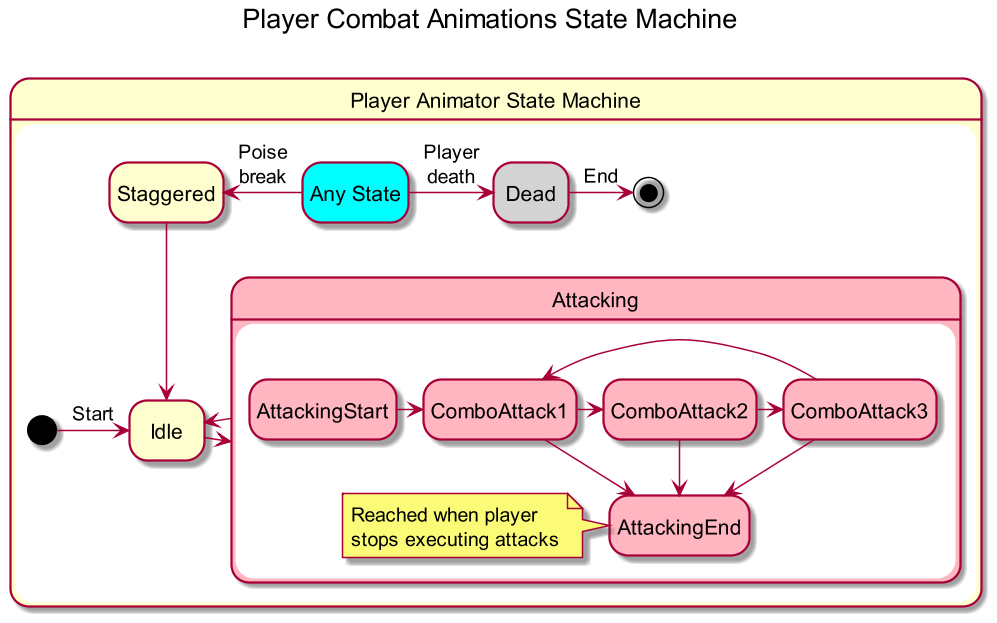
\includegraphics[width=34em]{figures/fig-player-anim-state-machine.png}
    \end{center}
    \legend{Source: Diagram assembled by authors.}
    \label{fig:player-anim-state-machine}
\end{figure}

%   > Hit detection toggled when receiving an event signal from the Attack animation
During Attack animations, the Animation System broadcasts event signals that toggle the activation and deactivation of the \emph{Hit Detection System}, which has the purpose of determining whether an attack successfully hit an enemy. At a certain point during the attack animation, we broadcast the \textsc{AttackCollisionStartEvent} which signalizes that attack collisions must be checked on each frame until an \textsc{AttackCollisionEndEvent} is signalized.

The \textsc{AttackCollisionEndEvent} is required to be signalized after the \textsc{AttackCollisionStartEvent} and before the attack animation ends so that attacks appropriately reflect what the attacking character performs. Generally, the point in time at which \textsc{AttackCollisionStartEvent} and \textsc{AttackCollisionEndEvent} are triggered should occur in the small time frame where the character swings the weapon in the direction of their target. Figure \ref{fig:attack-combo-diagram} shows the relationships between components involved in issuing Attack commands and handling combo states and animations.

% Figure: Attack and combos Class Diagram
\begin{figure}[!ht]
    \begin{center}
    \caption{A diagram showing the event flow and class relationship of the Attack and Combo related classes.}
    \vspace{0.5em}
        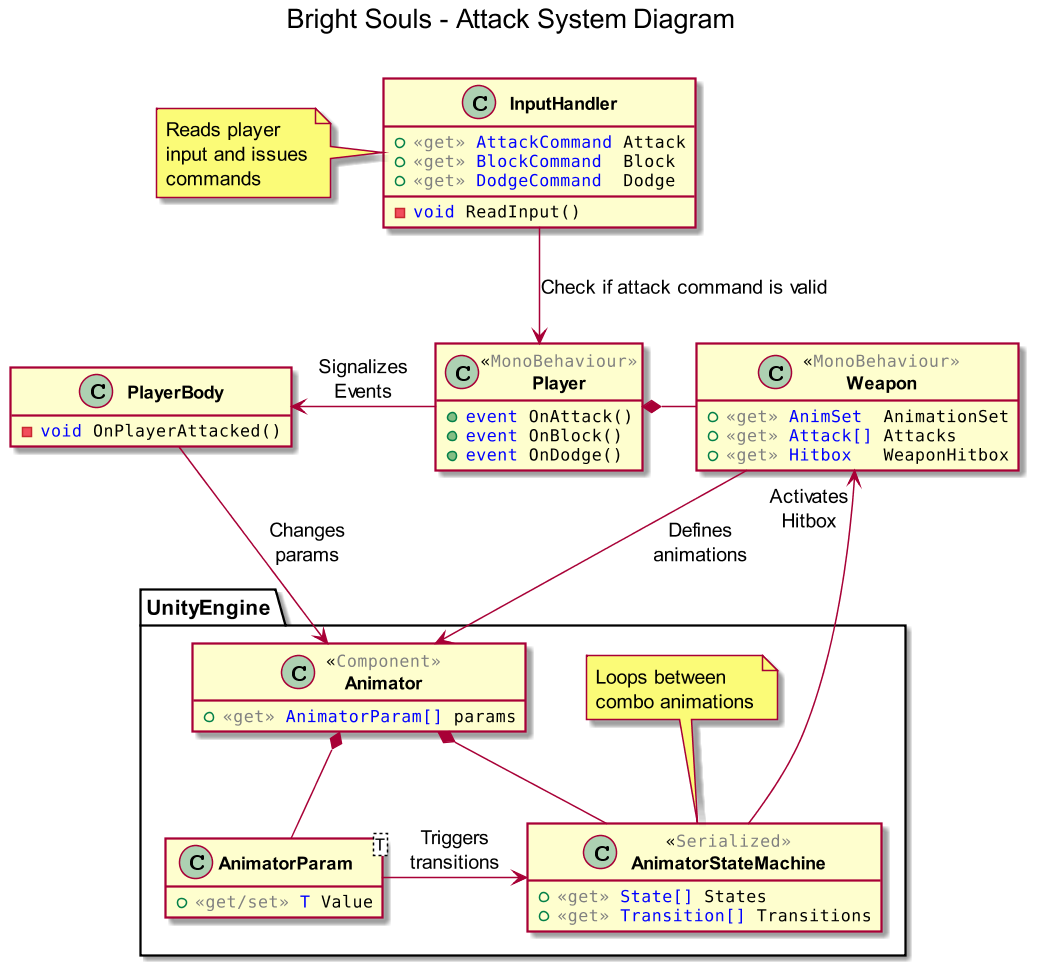
\includegraphics[width=34em]{figures/fig-attack-combo-diagram.png}
        \legend{Source: Diagram assembled by the authors.}
    \end{center}
    \label{fig:attack-combo-diagram}
\end{figure}

%     - Hit detection must not occur twice between the same target and same attack
%     - Specific collision layer to detect hitbox collision
To implement hit detection, we perform collider overlap checks in fixed time intervals of 16 milliseconds. These collision checks occur in a special collision layer called HitDetection, where every Collider is either the weapon of an attacker or the body of a target. This is an optimization requirement to meet the required time constraint in most computing systems. If a system is unable to meet the time constraint, there is a small chance that an attack might not be detected, where the attacker weapon "passes-by" the body of the attacker without triggering collision detection.

We estimate that attack collision detection occurs for approximately 20 frames from the point where it is first activated. Thus, if a computer system is able perform at least 4 updates per second, attack collision is guaranteed to be correctly detected. It is important to note that updates to the collision detection system are independent to the rendering performed by the graphics pipeline, and as a consequence are unaffected by most forms of temporary stutters in the application.

We also require safety measures to ensure that attack collision detection does not trigger a Hit event twice given the same Attack and Target entities. Therefore, for each attack performed by an attacking entity that is successfully registered as a Hit, we store a reference to an \emph{AttackCollision} instance in the \emph{Hitbox} component of the target entity. The Hitbox component then listens for the \emph{AttackCollisionEndEvent}, where the reference can be deleted since at this point the same \emph{AttackCollision} instance is not performing any collision checks.

% - Hit detection:
%   > Colliders:
%     - Hitbox overlap detection for attacker weapons and target character
%     - Attack Colliders are bounding boxes in weapons
%     - Character colliders are simplified bounding boxes that enclose torso, head and partially legs
For each occurrence of an attack collision, two colliders are obligatorily involved: one for the weapon of the attacker, and one for the body of the target. The colliders are instanced as \emph{bounding boxes}\sepfootnote{fn:bounding-boxes} that fully or partially enclose the 3D models of their relative entity. In order to perform collision checks with a reasonably optimized numbers of collision checks, we simplify bounding boxes of character models to only enclose the torso, head and a central position of the legs of a target. Using this method, we can minimize the amount of collision checks per frame, while also having appropriate precision for our implementation purposes.

%     - Consider character faction to recognize which combat characters can be hurt by an attack
After the collision detection step is performed, we must ensure that the attacking character is hitting a target that is not part of their own \emph{Combat Group} before validating an attack as a \emph{Successful Hit}. To do this we create the \textsc{FactionAttribute}, which determines that each character belongs to a combat group that is unable to perform attacks to other members of the same group. This is done so that groups of characters such as enemies of the player do not damage themselves when attempting to hit a target while being too close to each other. The values that the faction attribute can be assigned are described in table \ref{tab:table-faction-groups}. In addition, figure \ref{fig:hit-detection-diagram} shows the execution flow and class relationship of components used during the Hit Detection step.

% * Table: Values for the Faction Attribute
\begin{table}
    \begin{center}
      \caption{A description of the values that can be assigned to the \emph{Faction Attribute} of targets that are part of the Combat System in our implementation.}
      \label{tab:table-faction-groups}
      \rowcolors{2}{}{gray!25} % Alternate row colors
      \begin{tabular}{ >{\small}w{l}{3em} >{\small}w{c}{3em} m{25em} } % alignments and column size
        \addlinespace
        \toprule
        % Headings
        \bf Name    & \bf Id   & \bf Description                                              \\
        \midrule
        % 3D Models
        Player       &       0 & Player character. The player is a single entity and the sole 
                                 participant of this faction group.                           \\

        Enemy        &       1 & AI Agents that represent Enemies, which are hostile to the 
                                 player character.                                            \\

        NPC          &       2 & Non-Playable Characters. AI Agents which are not hostile to 
                                 the player character, but are hittable by and potentially 
                                 hostile to Enemies. An example of a Non-Playable Character 
                                 would be a companion which follows the player character and 
                                 aids them in combat encounters, being hostile to characters 
                                 belonging to the Enemy faction.                              \\

        Interactable &       3 & Static objects that can be attacked by the Player, Enemies or 
                                 Non-Player Characters and provide some type of feedback when 
                                 attacked. An example of an interactable entity would be a 
                                 barrel that can be attacked and destroyed.                   \\
        \bottomrule
      \end{tabular}
    \end{center}
\end{table}

% * Figure: Hit detection class diagram
\begin{figure}[!ht]
    \begin{center}
    \caption{Class diagram showing an overview of the components and flow of events related to the \emph{Hit Detection System}.}
    \vspace{0.5em}
        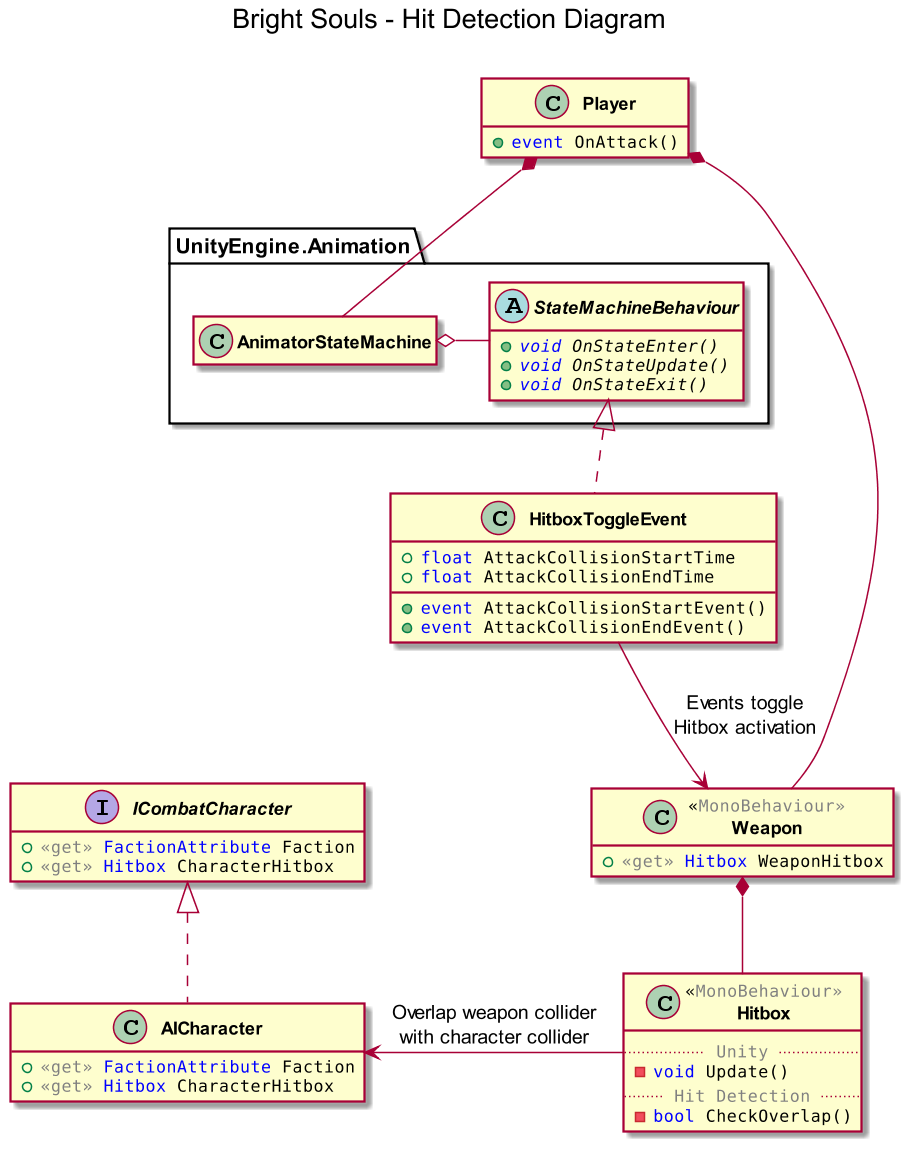
\includegraphics[width=30em]{figures/fig-hit-detection-diagram.png}
        \legend{Source: Diagram assembled by authors.}
    \end{center}
    \label{fig:hit-detection-diagram}
\end{figure}

% - Attack damage and other effects are abstracted into Combat effects
%     - Manipulate character attributes, statuses and physics
Once we performed all steps regarding the verification of whether an attack successfully hit an enemy, we can proceed to the next step of applying the \emph{Combat Effects} contained by the Attack. Combat Effects are our abstraction to the set of attribute effects, status effects and any other behaviors that occur when a character is struck by an attack. Examples of Combat Effects include the damage dealt to the Health of a target, Status effects such as \emph{Staggers}\sepfootnote{fn:stagger}, and physics effects such as the \emph{Knockback}\sepfootnote{fn:knockback} caused by an attack. Figure \ref{fig:combat-effects-diagram} shows an overview of the relationship between classes and components regarding the application of \textsc{CombatEffects} to \textsc{ICombatTarget} entities.

% * Figure: Combat Effect class diagram
\begin{figure}[!ht]
    \begin{center}
    \caption{Class diagram representing the relationships for Combat Effects and affected components.}
    \vspace{0.5em}
        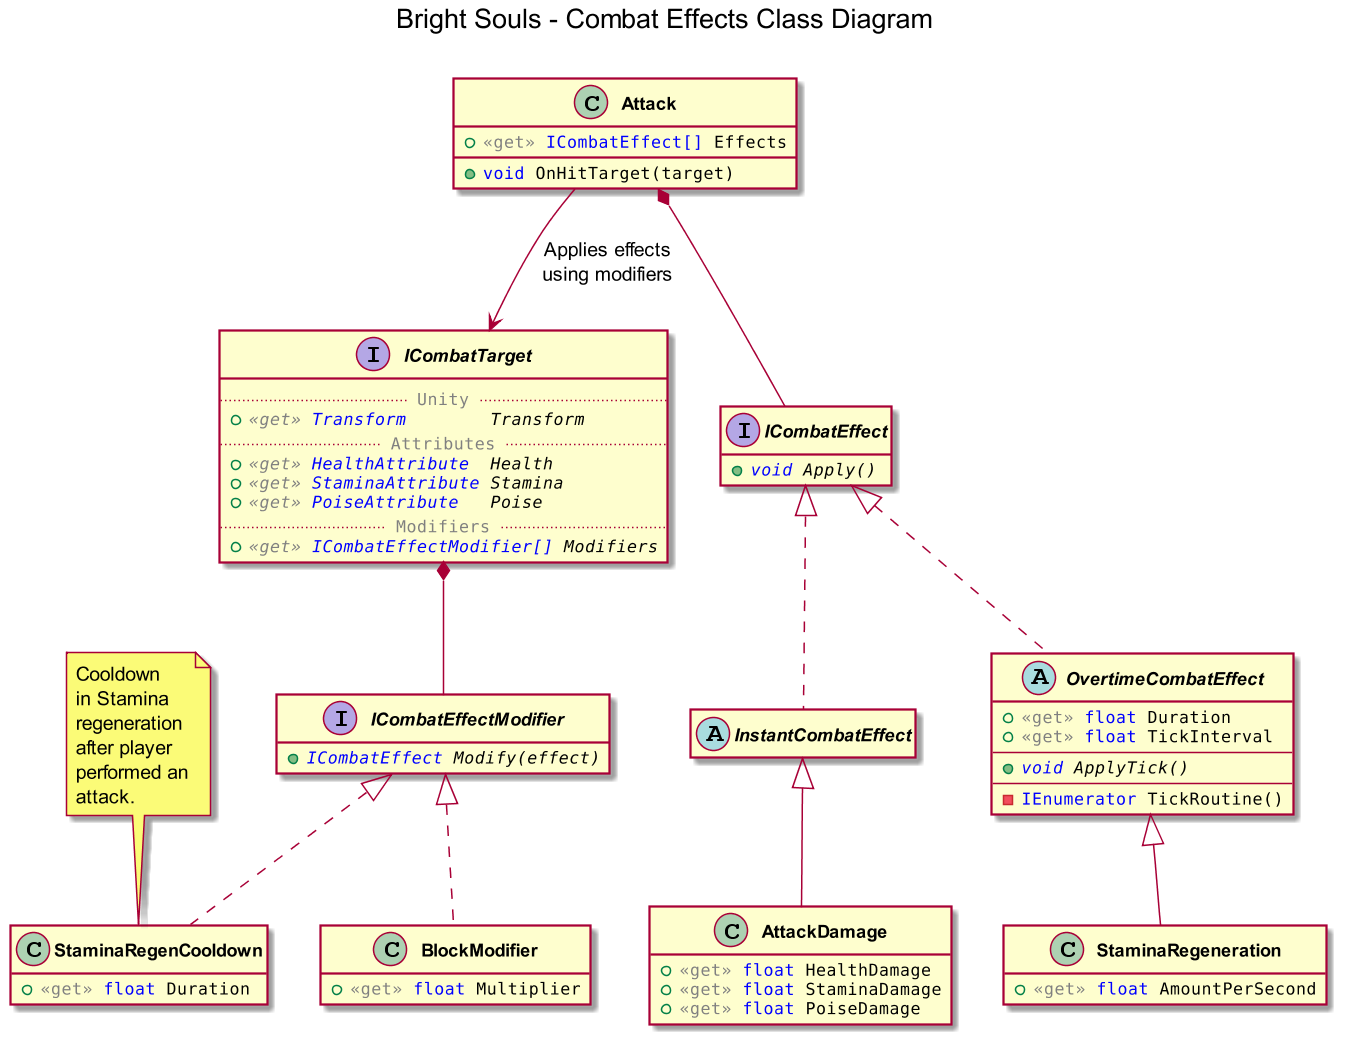
\includegraphics[width=32em]{figures/fig-combat-effects-diagram.png}
        \legend{Source: Diagram assembled by authors.}
        \label{fig:combat-effects-diagram}
    \end{center}
\end{figure}

%     - Instant combat effects are completely applied in the same frame as hit detection occurred
%     - Over-time combat effects with fixed interval ticks
In our implementation, we differentiate between \emph{Instant Combat Effects} and \emph{Over-time Combat Effects}. Instant Effects are applied to a target when a discrete event such as an attack takes place, and will often simply modify the value of an attribute. Examples of Instant Effects include the Health damage caused by an attack to a target and the Stamina cost of performing the attack, which is applied to the attacker. Over-time Effects are effects that occur in fixed time intervals over the course of a duration or is bound to the life of an entity.

% Player has a default Stamina regeneration effect
An example of Over-time effect would be the \textsc{StaminaRegeneration} effect that is permanently applied to the player, and which is temporarily blocked or modified by combat-related actions. During the course of a level, the player recovers a default amount of the Stamina resource over fixed time intervals, until either their Stamina resource is at the maximum possible amount or a combat action is performed. After a certain amount of time without issuing combat-related commands such as Attacking and Dodging, Stamina regeneration is re-enabled. Entering the Blocking state also modifies stamina regeneration by applying the \textsc{BlockingStaminaRegenModifier}, where the amount of stamina recovered is halved.

% - Combat Effect Modifiers
Combat Effects are restricted to performing modifications on a limited set of Attributes and Components exposed through the \textsc{ICombatTarget} interface, which is implemented by any entity that can be attacked. Before applying an effect to a target, we first check if the target contains any \emph{Combat Effect Modifiers}, such as a damage modifier caused by the target \emph{Blocking} or \emph{Dodging} an attack.

If the target has effect modifiers that are compatible with any of the effects being applied by an attack, the \textsc{Attack} class uses the modifiers to reconstruct its Combat Effects with updated values that reflect the purpose of the modifier. For instance, if the target successfully blocks an attack, the \textsc{BlockDamage} modifier is added to the target, which is used by the \textsc{Attack} class to update the \textsc{AttackDamage} combat effect by halving the damage that should be applied to the target. After the reconstruction of Combat Effects using any applicable modifiers, we finally commit to performing the attribute and status modifications and behaviors that are caused by an attack.

In figure \ref{fig:combat-flow-diagram}, we show an overview of all the steps involved with handling attacks, including detection of Attack commands being issued by the player, management of the animation states associated with weapons, validating Hitbox collision and combat groups with a Hit Detection System, and applying combat effects to modify target attributes and execute behaviors.

% * Figure: Flow of Combat System when processing Attack of entities
\begin{figure}[!ht]
    \begin{center}
    \caption{An event flow diagram that shows an overview of each step in our implementation of attacking in the Combat System.}
    \vspace{0.5em}
        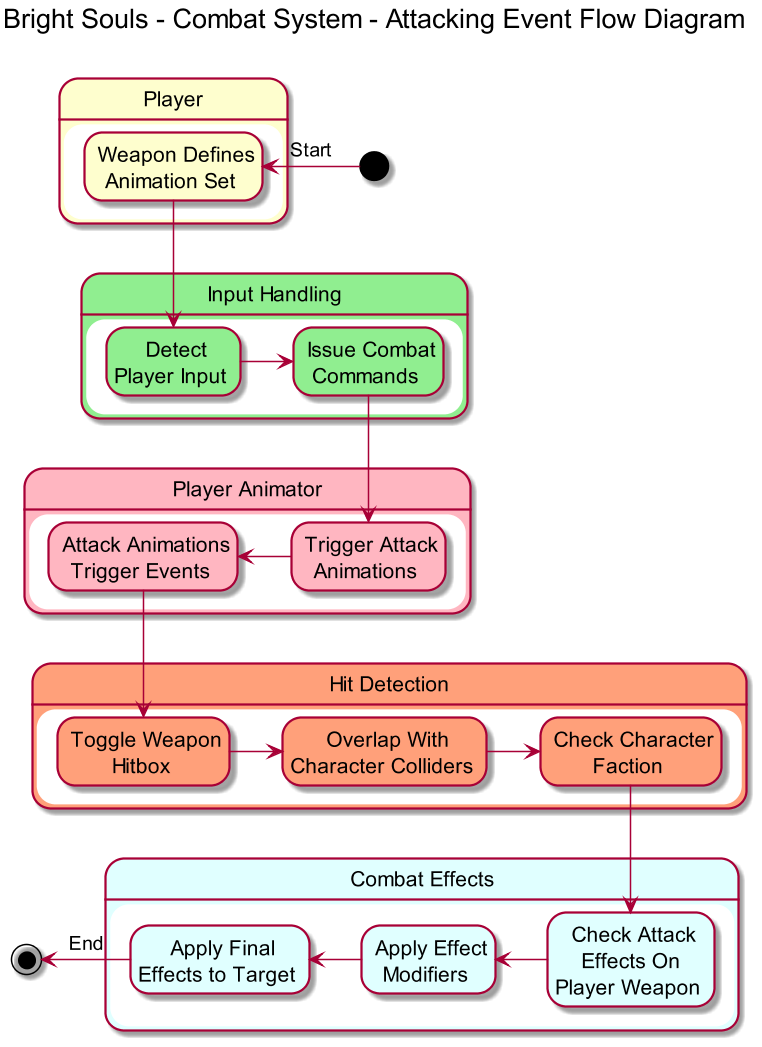
\includegraphics[width=22em]{figures/fig-combat-flow-diagram.png}
        \legend{Source: Diagram assembled by authors.}
    \end{center}
    \label{fig:combat-flow-diagram}
\end{figure}

%     - Block detection occurs when target is hit, is in "blocking" state and vector dot product between attack and target directions is < 0
To perform the blocking action, the player holds an input button which continuously issues the \textsc{BlockCommand}. When the player character is hit by an attack while performing the blocking action, we calculate the vector dot product between the attacker direction and the player direction before the player is hit. If the result has a negative value, it means that the player is pointing their shield towards the target, and thus it results in a successful block. If the target attacks the player from behind, the player is unable to block the attack.

% TODO (ADDITIONAL) Add formulae to vector dot product between defender and attacker direction, with outcomes.

%     - Dodge detection also occurs when target is hit. If hit detection occurs during target invincibility frames, a "dodge" is registered, and target receives no combat effects
Contrary to blocking, the \textsc{DodgeCommand} is issued discreetly at the press of a button. When the player presses the dodge command, the \textsc{Player} component signalizes the action to the animation system. If the player issues the command when moving towards a specific direction, the \textsc{Animator} component handles the movement of the \textsc{Transform} to translate the character into that direction. If the player is stationary when the dodge command is issued, the \textsc{Animator} simply uses the current direction defined by the \textsc{Transform}.

Over the duration of the dodge animation, we issue the \textsc{DodgeIFramesBegin} and the \textsc{DodgeIFramesEnd} events, which toggle the \textsc{Invincibility} combat effect modifier to the player. The Invincibility combat effect nullifies any negative combat effects that might affect the player during an attack, causing enemy attacks to have essentially no effect over the player.


% ============================================================================
% ============================================================================
% ============================================================================

% TODO \subsubsection{Animation System (ADDITIONAL)}

% Animation system
% - Difference in body movement when in Orbital vs Lock-On Cameras
% - React to attribute changes, motor velocity and physics updates

% - Figure: Player Animation State Machine

% - Statuses such as staggered, dead will override other animations
% - Blending between animations states when performing directional actions
% - Transitioning between combo states
% - Animation events for hit detection when attacking

% - Figure: Animation System class diagram showing component relations and events

% ============================================================================
% ============================================================================
% ============================================================================

\section{Artificial Intelligence and Enemy Design}

% Enemies in Dark Souls present basic, somewhat predictable behavior (REF Analysis Dark Souls)
As discussed in \ref{sec:analysis-dark-souls}, enemies in Dark Souls present basic and somewhat predictable behavior. When spawned, enemies either remain stationary or move through predefined paths until interaction with the player. When detecting player presence, they will often switch to a combat stance where they perform an attack from a limited and small set, and then switch to a defensive stance for the duration of a \emph{Cooldown}\sepfootnote{fn:cooldown} timer.

%   - Decided to use State Machines to replicate simplistic behavior
While we were unable to gather any specific information on how \emph{AI Agents} are implemented in the source code of Dark Souls, we argue that \emph{State Machines} can be used to implement the behaviors we observed and described. Using State Machines, we can represent the actions performed by enemies in Dark Souls as \emph{States} and \emph{Behaviors}. Each enemy will be in a particular State at a given point in time, and each State contains a set of behaviors that define the actions performed by an agent given environmental and player-related circumstances.

% ============================================================================
% ============================================================================
% ============================================================================

\subsection{State Machines}

To exemplify our claim, when an enemy is stationary we consider it to be in the \emph{Idle} state, which contains no particular Behaviors attached to it. When an enemy is moving along predefined paths and scouting for the player it is considered in the \emph{Patrolling} state, which contains the \emph{Scan} Behavior, which checks for the presence of the player in an area near the enemy, and the \emph{WaypointMovement} Behavior, which handles movement of the entity. Figure \ref{fig:fig-ai-state-machine} shows an example of a State Machine definition which is used by Melee-range enemies in our implementation, such as the \emph{Ghouls} and \emph{Warrior Skeletons}.

% * Figure: Melee enemy AI State Machine
\begin{figure}[!ht]
    \caption{An example of the State Machine that represents a Melee Enemy AI Agent. Each state holds its own behavior.}
    \begin{center}
        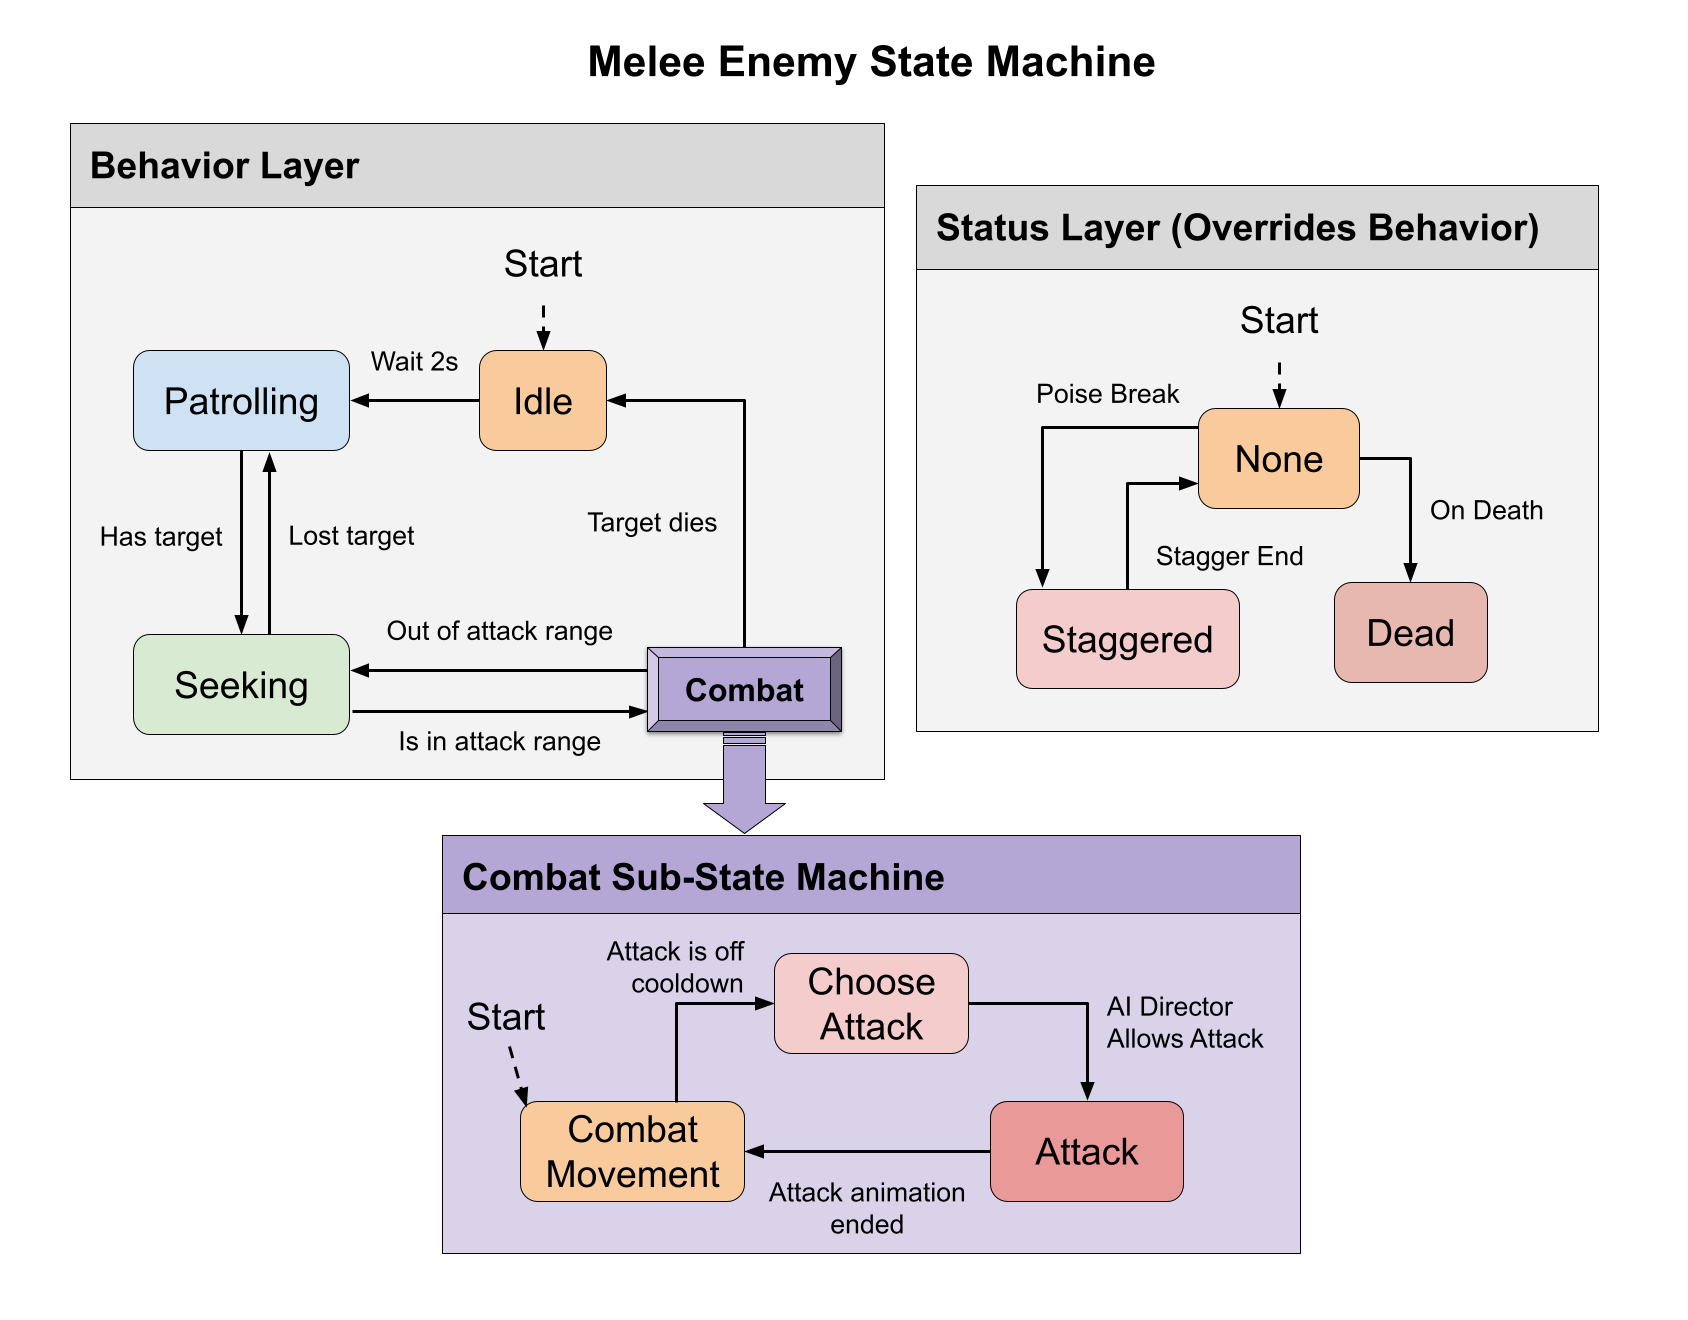
\includegraphics[width=34em]{figures/fig-melee-ai-state-machine.png}
    \end{center}
    \legend{Source: Diagram assembled by authors.}
    \label{fig:fig-ai-state-machine}
\end{figure}

% Implementation of a Serializable, multipurpose State Machine structure
%   - StateMachineController: MonoBehaviours, instanced in scenes. Contains a reference to the state machine and its owner. Validates conditions for transitions, performs transitions and updates states.
For our implementation, we use a generic definition of State Machines which can be used outside the scope of implementations of AI Agents. We start by defining a \textsc{StateMachineController} component which can be assigned to a MonoBehaviour. In the context of AI Agents, the StateMachineController will be attached to an \textsc{AICharacter} component, which represents the root hierarchy level of AI-controlled characters. The \textsc{StateMachineController} contains a reference to the \textsc{StateMachine} and to its owner, and is tasked with performing frame-bound updates to states and validating the conditions to perform transitions between states. Therefore, the \textsc{StateMachineController} is the sole runtime component in our State Machine implementation.

% - State Machines are bound to asset files
% - Class Definitions:States, Transitions, StateBehaviors
%   - StateMachine: Class definition for all the serialized data involving our implementation of state machines. Contains states and transitions. 
%   - States: Contain a variable set of Behaviors, that can be assigned dynamically during runtime and serialization.
%   - Transitions: References an origin and a target state, and contains a set of boolean conditions to validate a transition as valid.
The definitions of State Machine, including their States, Transitions and Behaviors are constrained to serializable space, with State Machines being bound to asset files that can be referenced to by the \textsc{StateMachineController}. The \textsc{StateMachine} class contains serialization data for \textsc{States}, which contain a variable set of \textsc{Behaviors}; and textsc{Transitions}, which contain references to an origin and target state and a set of boolean conditions to define when the transition should occur. Figure \ref{fig:state-machine-class-diagram} shows the class and data structure relationships for our implementation of state machines.

% * Figure: State Machine system architecture
\begin{figure}[!ht]
    \begin{center}
    \caption{Class relationship for our State Machine implementation from the perspective of AI Systems.}
    \vspace{0.5em}
        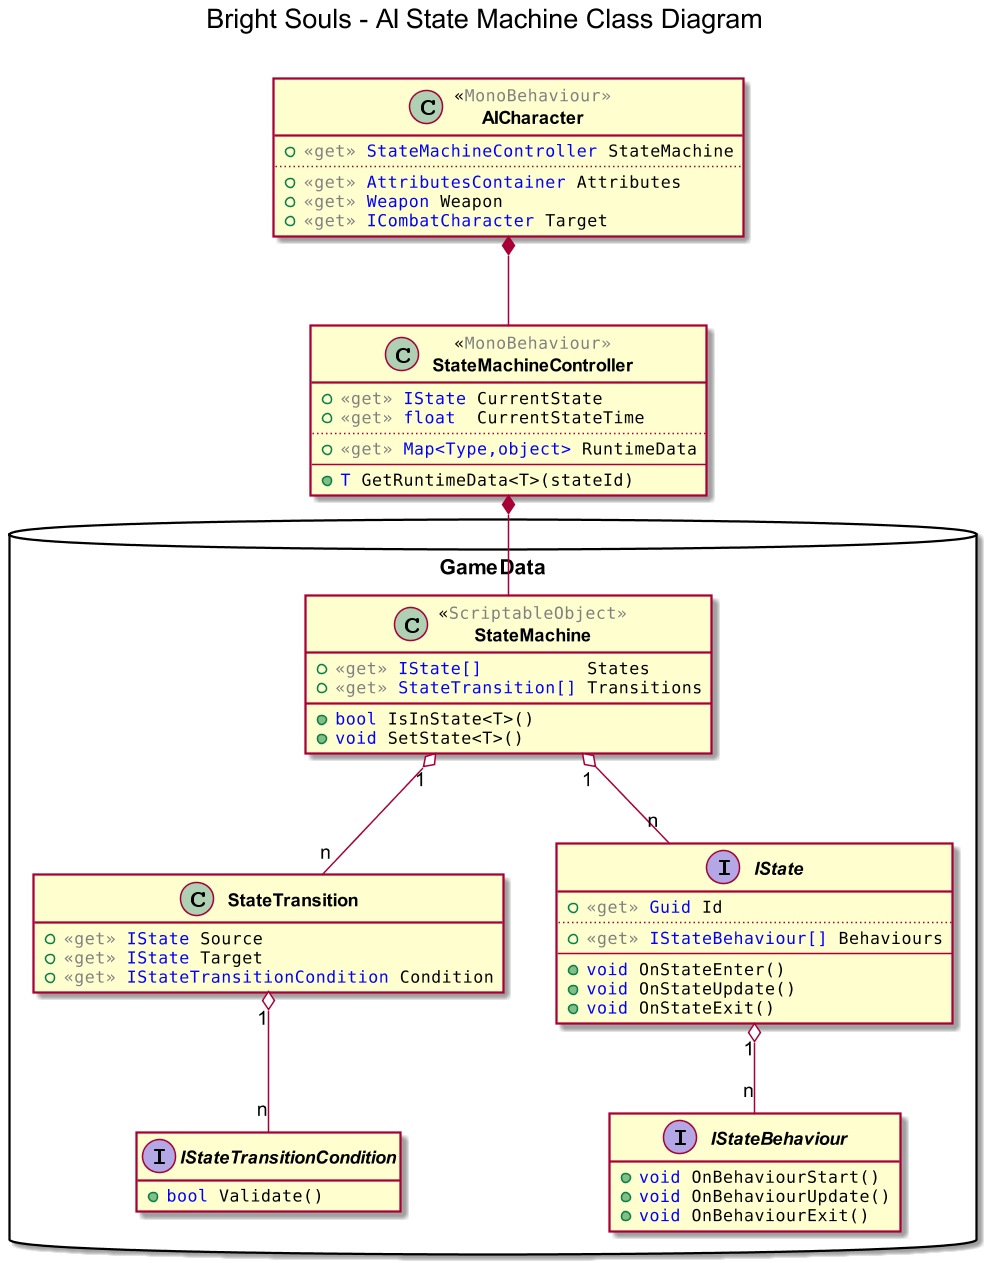
\includegraphics[width=28em]{figures/fig-state-machine-class-diagram.png}
        \legend{Source: Diagram assembled by authors.}
    \end{center}
    \label{fig:state-machine-class-diagram}
\end{figure}

% Each state has a set of dynamically assigned Behaviors that determine the actions performed by an AI Agent on that state.
Each \textsc{State} has a set of dynamically assignable \textsc{Behaviors}, which determine the actions that are performed by the AI Agent that contains the State Machine. In table \ref{tab:ai-behaviors}, we define all the possible behaviors in our implementation, specifying the States in which they are used and a brief description of the actions performed by the AI Agent when executing the Behavior.

% * Table - AICharacter Behaviors
% =================================================================================
% Name           | Related States   | Description
% =================================================================================
% WaypointMove   | Patrolling       | Uses a set of waypoints (which can be empty)
%                |                  | to move a character in fixed points on the
%                |                  | NavMesh of the environment.
% ---------------|------------------|----------------------------------------------
% Scan           | Idle, Patrolling | Uses a set of collision triggers to detect
%                |                  | enemies of the AI agent in an area around or
%                |                  | in front of its position, and assigns a 
%                |                  | target upon detection.
% ---------------|------------------|----------------------------------------------
% Seek           | Seeking          | Follows a target, constantly moving to its
%                |                  | position until the target is out of range.
% ---------------|------------------|----------------------------------------------
% AdjustDistance | CombatMovement   | Adjusts the distance of the AI Agent to be
%                |                  | close enough to perform an attack, without
%                |                  | being too close to the target.
% ---------------|------------------|----------------------------------------------
% PlanAttack     | CombatMovement   | Chooses the next attack based on the actions
%                |                  | being performed by the target, or by using
%                |                  | random number generation.
% ---------------|------------------|----------------------------------------------
% Attack         | CombatMovement   | Performs the chosen attack on the target
%                |                  | using the Attack System pipeline.
% ---------------|------------------|----------------------------------------------
% RotateAttack   | CombatMovement   | Performs body rotation to adjust the attack
%                |                  | to a moving target. The rotation has limited
%                |                  | speed to permit the target to dodge.
% ---------------|------------------|----------------------------------------------
% Shoot          | Shooting         | Used by ranged enemies. Continuously shoot
%                |                  | arrows at a target until the target is
%                |                  | out of range.
% ---------------|------------------|----------------------------------------------
% Death          | Dead             | Deactivates all components, triggers the
%                |                  | death animation and de-spawns the AI agent.
% =================================================================================

\begin{table}[!h]
    \begin{center}
      \caption{A list of the behaviors in the States of the AI Agents in our implementation.}
      \label{tab:ai-behaviors}
      \rowcolors{2}{}{gray!25} % Alternate row colors
      \begin{tabular}{ >{\small}w{l}{6em} >{\small}w{l}{7em} >{\small}m{17em} } % alignments and column size
        \addlinespace
        \toprule
        % Headings
        \bf Name       & \bf Related States  & \bf Description                              \\
        \midrule
        WaypointMove   & Patrolling          & Uses a set of waypoints (which can be empty)
                                               to move a character in fixed points on the 
                                               NavMesh of the environment.                  \\
        Scan           & Idle, Patrolling    & Uses a set of collision triggers to detect   
                                               enemies of the AI agent in an area around
                                               or in front of its position, and assigns a 
                                               target upon detection.                       \\
        Seek           & Seeking             & Follows a target, constantly moving to its
                                               position until the target is out of range.   \\
        AdjustDistance & CombatMovement      & Adjusts the distance of the AI Agent to be 
                                               close enough to perform an attack, without
                                               being too close to the target.               \\
        PlanAttack     & CombatMovement      & Chooses the next attack based on the actions 
                                               being performed by the target, or by using
                                               random number generation.                    \\
        Attack         & CombatMovement      & Performs the chosen attack on the target 
                                               using the Attack System pipeline.            \\
        RotateAttack   & CombatMovement      & Performs body rotation to adjust the attack 
                                               to a moving target. The rotation has limited 
                                               speed to permit the target to dodge.         \\
        Shoot          & Shooting            & Used by ranged enemies. Continuously shoot 
                                               arrows at a target until the target is 
                                               out of range.                                \\
        Death          & Dead                & Deactivates all components, triggers the 
                                               death animation and de-spawns the AI agent.  \\
        \bottomrule
      \end{tabular}
    \end{center}
  \end{table}

% State machines are serialized, therefore Behaviors are unable to keep state of objects that are instanced in a scene. We need to keep data for each behavior in the container of the state machine, which in this case is the AICharacter.
States are serialized and independent of any instanced objects, which in consequence creates the restriction that Behaviors are unable to store any type of runtime data from instanced entities, or even static data that is referenced by the entities. Therefore, we are required to maintain the data used by each behavior in the container of the \textsc{StateMachineController}. For this reason we create the \textsc{IStateMachineOwner} interface, which provides a public accessor to a \textsc{Hashmap} structure which contains the runtime and referenced data for an instanced entity, using an identifier for the current state as the \emph{Key}.

% ============================================================================
% ============================================================================
% ============================================================================

\subsection{Implementation of Behaviors}

% Movement:
%   - Use of NavMeshes to define walkable space in 3D environment for AI Agents.
%   - Use of A* path-finding algorithm to define movement over nodes scattered throughout the mesh.
For an AI Agent to perform movement over the environments that were assembled when executing the \textsc{WaypointMove} or \textsc{Seek} behaviors we use Unity's \emph{NavMesh} system, which uses the topology of 3D objects and a user-defined set of layers with movement costs to generate a simplified mesh representing the traversable ground in the environment. The resulting mesh also contains weights for each vertex, which causes the AI Agent to prioritize certain paths defined by the user. Using the data generated from \emph{NavMeshes}, we define the movement performed by the AI as a set of waypoints that are calculated using the \textsc{A*} algorithm with the \textsc{Manhattan Distance} heuristic.

% How AI agents scan for targets
% - Spheric collider for frontal view cone
%      - Detects collision with ICombatCharacters from different Faction
% - Calculate the angle between agent forward and target relative pos
To scan for targets in the environment, AI Agents have a spheric collider representing the radius where a target can be detected by a frontal view cone. The collider detects collision with \textsc{ICombatCharacter} entities where the \textsc{FactionAttribute} has a different value to that of the agent. If a target is within this radius, we calculate the angle between the forward vector\sepfootnote{fn:forward-vector} of the agent and the relative direction of the target. The forward vector is natively supplied by \textsc{Unity} with the \textsc{Transform} component, but we also need to project the vector onto the two-dimensional [X, Z] plane.

% - How target relative pos is calculated
% - Use of another, smaller spheric collider for enemy hearing
The \emph{Target Relative Direction} is calculated by subtracting the target position to the position of the agent, normalizing the result and projecting it onto the ground plane. Having these vectors, we use the \textsc{Vector3.Angle} operation from \textsc{Unity} to clamp field detection range to a cone of 90 degrees, causing the agent to have a constrained field of view. Additionally, we use another spheric collider with smaller radius to represent the distance in which the AI Agent would be able to hear. When an entity of the type \textsc{ICombatCharacter} enters this collider, the AI Agent will immediately consider it as the new target.

% - What happens when the target dies
%       - AI agent is reset to Idle
% - If target is unreachable, same thing happens
When the target dies, the AI agent is reset to their default state - which is generally the start point of its state machine. Therefore, when an enemy AI agent is able to defeat the player, they will return to the \emph{Idle} state. A similar event happens when the AI agent is in the \emph{Seeking} state and the target can not be interacted with. If the target is in an unreachable position where there is no path connecting the ground NavMesh from agent to player position, the AI loses interest in the target and returns to its default state.

% How AI Agents attack
%   - Each enemy has own state machine
%   - State state differs because of behaviors and data
%   - CombatMovement: adjust position, plan attack, execute
In our implementation, we group AI agents by an \emph{Enemy Type}. Each enemy type will have its own State Machine definition. While the State Machine for an enemy type might contain states with the same name as another, their functionality differs by using a different set of behaviors or different values for the data in the behaviors. The most relevant example would be in the \textsc{CombatMovement} state where a melee AI agent must adjust their position, plan their attack and perform the attack based on their position in the environment, their available actions and the actions being performed by the player. The \textsc{CombatMovement} state is functionally the same as the sub-state machine concept used in hierarchical state machines. We switch between three unique behaviors to give the impression of different states: \emph{PositionAdjustment}, \emph{AttackPlanning} and \emph{AttackExecution}.

% AdjustPosition
%     - Two-dimensional radial and distance-based positioning
In the \textsc{PositionAdjustment} behavior, we have several steps to calculate the position an AI agent should move towards. We start by defining a two-dimensional vector to define the position an AI agent should be in relative to their target: a \emph{distance relationship} between the agent and their target and a \emph{radial-distribution} position, where the agent positions itself in a circular perimeter around the target.

%     - GroupAIBrain: What is the expected distance?
To define the distance relationship between the agent and their target, we consider parameters that define the context of the combat encounter. First, we communicate with the \textsc{GroupAIBrain} component to understand whether the player is dealing with too many enemies, which means the agent should take a more idle stance and remain in the backline. The \textsc{GroupAIBrain} component is a manager to all AI agents engaged in a \emph{Combat Encounter} against the player.

\sepfootnotecontent{fn:hitbox-central-point}{Footnote: What is the hitbox central point?}

%     - Is the attack in cooldown?
%     - Distance to Player: Would an attack hit?
Second, we determine if the AI agent attacks are on \emph{cooldown}, meaning that the agent is not able to attack for a short period of time after performing another attack. If so, the agent takes a defensive approach and attempts to position itself further away from the player so that the player has to make a time investment to be able to attack the agent. Third, we calculate the average \emph{Hitbox Central Point}\sepfootnote{fn:hitbox-central-point} distance for all attacks that the AI Agent can perform. We use this average to create a target position that minimizes the chances of the player being able to avoid an attack by simply moving backwards. This step is performed when the target is either out of attack range or after half of the \emph{cooldown} duration for the next attack.

% - GroupAIBrain: What is the expected radial position?
%     - Priority index
%     - Positions in arc in circular perimeter
%     - Arc boundaries restricted by environment geometry
%     - Arc also restricted by dynamic radian in GroupAIBrain
To define the radial-distribution position for an entity, the AI Agent is assigned a numeric priority index upon entering a \emph{Combat Encounter} instance against the player. The value of the priority index is used to evenly arrange AI Agents in a constrained arc of a circular perimeter around the player. The aperture of the arc is defined by both the geometry of environment colliders around the player and adjustment metrics. If the arc boundaries are not restricted by environmental geometry, the aperture is defined by an adjustable radian supplied by the \textsc{GroupAIBrain} component.

% - How agents are distributed in the arc
% - Arc divided in equal size segment
% - First agent in center
% - Second and third agent in boundaries
The agent placement arc is divided in equal size segments that are used to distribute the agents uniformly in relation to the player. At the beginning of a combat encounter, a single agent becomes part of the AI group. This initial agent is defined as the pivot for the group. The arc is divided in two segments by the position of the pivot agent, which is exactly at the center of the two segments. The following two agents are placed at the outer boundaries of the arc, each at the limits of their respective segments.

% - Subsequent agents subdivides largest segments from center outwards
% - Recalculate segments when agents die
Every subsequent agent subdivides the largest segment that is closest to the pivot, using the center position of the segment and creating two new segments. When the pivot agent is defeated, a new pivot agent is selected based on its distance from the original pivot, and the segments are recalculated by adding each subsequent agent that is closest to the pivot through the same algorithm. When non-pivot agents are defeated, the group is also recalculated but with the difference that we use the same pivot when recalculating agent segments. This algorithm is exemplified by figure \ref{fig:arc-segments}, and the resulting behavior can be seen in figure \ref{fig:enemy-positioning-example}.

% * Figure: Figure illustrating the behavior of the "arc segments" algorithm
\begin{figure}[!ht]
    \caption{Illustration of the "Arc Segments" algorithm for radial positioning of AI Agents around the player character.}
    \begin{center}
        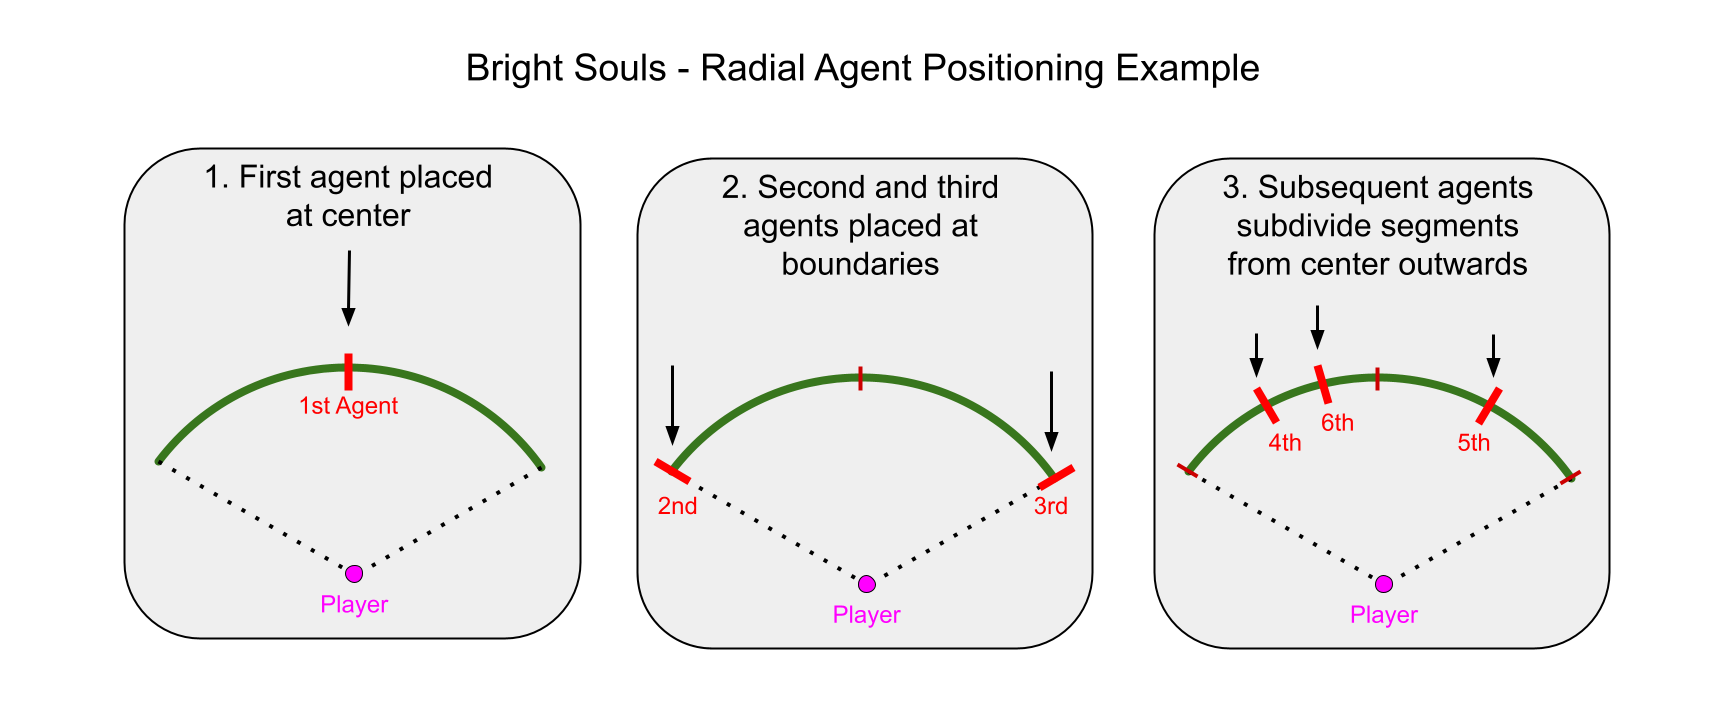
\includegraphics[width=32em]{figures/fig-arc-segments.png}
    \end{center}
    \legend{Source: Diagram assembled by authors.}
    \label{fig:arc-segments}
\end{figure}

% * Figure: Enemy typical radial placement around the player character
\begin{figure}[!ht]
    \caption{An example of melee enemy group positioning with five AI Agent enemies.}
    \begin{center}
        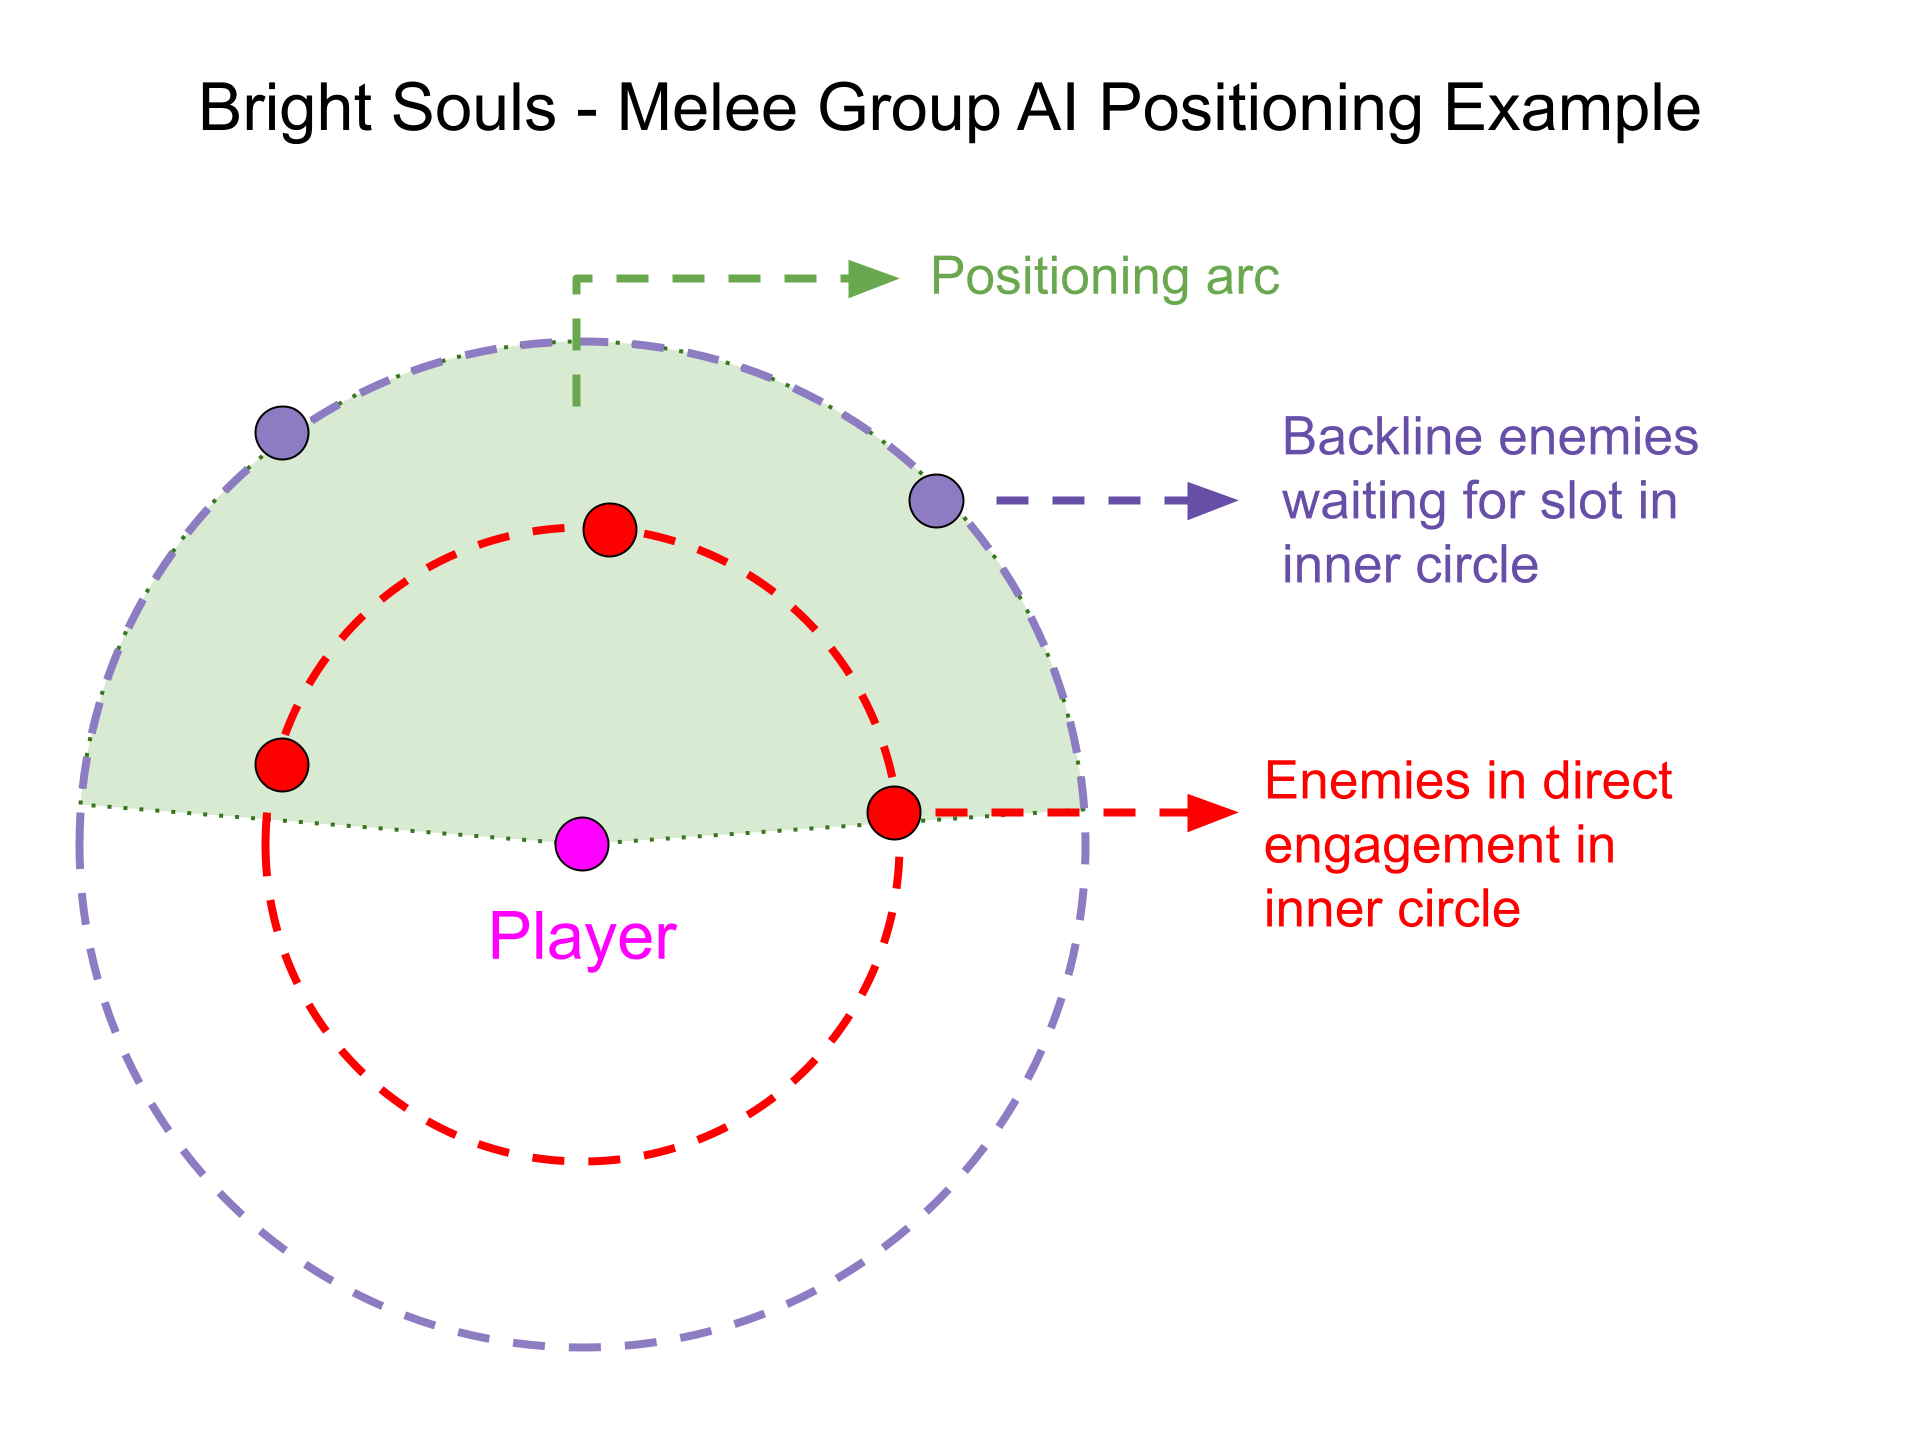
\includegraphics[width=26em]{figures/fig-enemy-positioning-example.png}
    \end{center}
    \legend{Source: Diagram assembled by authors.}
    \label{fig:enemy-positioning-example}
\end{figure}

% PlanAttack behavior
% Player State + GroupAIBrain info used as input
% Decide if can attack and which attack
In the \textsc{PlanAttack} behavior, we use information from player state along with constraints imposed by the \textsc{GroupAIBrain} component to define if an attack can be executed, and which attack the AI Agent should perform at a given context. Each attack has a different purpose designed to guide the player towards a specific response.

%     - AI Brain: Does it give permission to attack?
%     - EGCD: Enemy Group Cool-Down
First, we query the \textsc{GroupAIBrain} component to check whether the current AI Agent being processed has permission to attack. Enemy AI Groups have a shared set of \emph{Enemy Group Cooldown} timers that are reset every time an AI agent performs an attack. All AI Agents that are part of a group will be unable to attack unless at least one of the available cooldown timers has a specific amount of elapsed time. Both the numbers of timers available and the minimum elapsed time for each are determined by adaptive parameters from the \textsc{GroupAIBrain} component, and are further discussed in section \ref{sec:adjustments}.

% Uses list of available types to query for information
%     - AI Brain: does it give permission for special attack?
Second, the PlanAttack behavior uses information on the available attack types to query which information is necessary to decide the attack. We communicate with the \textsc{GroupAIBrain} component to determine if the entity is able to perform \emph{Special Attacks}. Given a small interval of time, a limited number of non-basic attacks can be performed by an agent. If the agent is unable to perform a Special Attack after querying availability from the \textsc{GroupAIBrain} component, it simply chooses one of multiple basic attacks to perform.

Non-basic attacks have the purpose of creating incentive for the player to perform a new or specific reaction. For instance, the \emph{Overhead} and \emph{Pierce} attacks are designed to punish the player if attempted to be blocked and drain their Stamina resource. If the player does attempt to block one of such attacks, they will quickly find themselves out of Stamina and trigger a \emph{Poise Break}\sepfootnote{fn:poise-break}.

%     - Is the player out of attack range?
%     - How often does the player back-step
Then, we check if the player is still out of attack range even after the adjusting its position during the PositionAdjustment behavior. If so, we use a parametrized threshold related to the chance of an agent performing a \emph{Charge} attack, if it is one the available movements. The threshold is combined with a \emph{profile} metric regarding the frequency the player uses back-steps to avoid attacks, and then used as input for a RNG (random number generation) algorithm to determine if the agent will perform the \emph{Charge} attack. The parametrized thresholds for each attack type are explained further in section \ref{sec:adjustments}. If the agent is not able to perform the \emph{Charge} attack, it is reverted back to the \emph{PositionAdjustment} behavior.

%         - Is the player blocking?
%         - How often does the player block, dodge?
In the same sense, we check if the player is blocking and use a threshold related to the chance of the agent performing an \emph{Anti-Block} attack, such as the \emph{Overhead} or \emph{Pierce} attacks. We combine that chance with the player \emph{profile} metric regarding the frequency which the player uses the Block Action to mitigate the damage of attacks, and use these values as input for the RNG algorithm to determine if the agent will perform an \emph{Anti-Block} attack. Anti-dodge attacks use a similar threshold adjustment system, with the exception that it is not considered whether the player is performing a dodge or not. Since the dodging action is discrete and occurs in a fraction of a second, the agent has to be able to predict when a player would perform a dodge so that the attack punishes the player.

% ============================================================================
% ============================================================================
% ============================================================================

% TODO \subsubsection{Management of Agent Groups}
%\label{sec:ai-brain}

% ============================================================================
% ============================================================================
% ============================================================================

% TODO \subsection{Design of Enemy Types (ADDITIONAL)}

% TODO Table - Enemy Types
%
% =========|============|========|===========|=========|==========================================
%  Name    | Move Speed | Damage | Atk Speed | Health  | Description                             
% =========|============|========|===========|=========|==========================================
% Ghoul    | Slowest    | Lowest | Slow      | Lowest  | Slow and weak enemy. Introductory enemy 
%          |            |        |           |         | for player to test mechanics.
% ---------|------------|--------|-----------|---------|------------------------------------------
% Skeleton | Fast       | Low    | Medium    | Low     | Fast enemy. Causes player to reposition 
%          |            |        |           |         | and protects archers.                  
% ---------|------------|--------|-----------|---------|------------------------------------------
% Warrior  | Slow       | Medium | Slowest   | High    | Uses shield. Hard to kill. Buys time for  
%          |            |        |           |         | all other enemies.  
% ---------|------------|--------|-----------|---------|------------------------------------------ 
% Archer   | Stationary | Low    | Slowest   | Medium  | Meant to slowly drain player health from
%          |            |        |           |         | a distance if not prioritized.           
% ---------|------------|--------|-----------|---------|------------------------------------------
% Knight   | Medium     | High   | Fast      | Highest | Meant to force player to dodge, blocking 
%          |            |        |           |         | his Attacks Drain too much Stamina.      
% =========|============|========|===========|=========|==========================================

% TODO Table - Attack Speed Values (tab:attack-speed-values)
%
% ==========|======|===========
% Atk Speed | APS  | Entities
% ==========|======|===========
% Slowest   | 0.33 | Archers,
%           |      | Warriors
% ----------|------|-----------
% Slow      |  0.5 | Ghouls
% ----------|------|-----------
% Medium    |  0.8 | Skeletons
% ----------|------|-----------
% Fast      |  1.5 | Knights
% ----------|------|-----------
% Fastest   |  2.3 | Player
% ==========|======|===========

% TODO Table - Health Values (tab:enemy-health-values)
%
% ========|======|===========
% Health  | PATK | Entities
% ========|======|===========
% Lowest  |    2 | Ghouls
% --------|------|-----------
% Low     |    3 | Skeletons
% --------|------|-----------
% Medium  |    6 | Archers
% --------|------|-----------
% High    |    8 | Warriors
% --------|------|-----------
% Highest |   10 | Knights
% ========|======|===========

% TODO Table - Damage Values (tab:enemy-damage-values)
%
% =======|======|===========
% Damage | ATKP | Entities
% =======|======|===========
% Lowest |   20 | Ghouls
% -------|------|-----------
% Low    |   14 | Archers, 
%        |      | Skeletons
% -------|------|-----------
% Medium |   12 | Warriors
% -------|------|-----------
% High   |    9 | Knights
% =======|======|===========

% TODO Table - Attack Types (tab:enemy-attack-types)
%
% =========|============|==========|===============================
% Name     | Type       | Enemies  | Description
% =========|============|==========|===============================
% Slash    | Basic      | Ghoul,   | Low damage attack, no health
%          |            | Skeleton | damage when blocked. Low poise
%          |            |          | damage.
% ---------|------------|----------|-------------------------------
% Arrow    | Basic      | Archer   | Low damage attack, no damage
%          |            |          | when blocked.
% ---------|------------|----------|-------------------------------
% Double   | Basic      | Knight   | Medium damage attacks, low 
% Slash    |            |          | damage when blocked.
% ---------|------------|----------|-------------------------------
% Charge   | Gap Closer | Skeleton,| Medium damage attack. Enemy
%          |            | Knight   | runs to player to land the
%          |            |          | attack from a long distance.
% ---------|------------|----------|-------------------------------
% Overhead | Anti-Block | Warrior  | Medium damage attack. Consumes
%          |            |          | half of player stamina if
%          |            |          | attempted to be blocked.
% ---------|------------|----------|-------------------------------
% Pierce   | Anti-Block | Knight   | High damage attack. Pierces
%          |            |          | through player defense, 
%          |            |          | consuming most of player
%          |            |          | stamina if blocked.
% ---------|------------|----------|-------------------------------
% Sweep    | Anti-Dodge | Knight   | Medium damage attack. Has
%          |            |          | three hit detection phases
%          |            |          | and a long duration. Meant
%          |            |          | to catch the player in the
%          |            |          | final position after a dodge.
% =========|============|==========|===============================

% ============================================================================
% ============================================================================
% ============================================================================

% TODO \subsection{Level Design (ADDITIONAL)}

% ============================================================================
% ============================================================================
% ============================================================================

% TODO \subsection{Audio and Visual Effects (ADDITIONAL)}

% ============================================================================
% ============================================================================
% ============================================================================

% TODO \subsection{User Interface (ADDITIONAL)}

% ============================================================================
% ============================================================================
% ============================================================================

\section{Telemetry and Performance Tracking}

To perform difficulty adjustments that satisfy the skill level and knowledge of a player regarding our implementation, we need to capture data regarding to how the game is being played. We then must use the data to reconstruct an order of events and analyze the patterns and outcomes of player actions, to determine if the player is being overtly successful or failing to meet the requirements of the challenged that was imposed by the current difficulty.

We use the previously discussed definition of player \emph{profile} and \emph{performance} to implement various metrics which represent the outcomes of actions performed by the player during a play session. Then, we use such metrics as an input to a comparison with predefined thresholds, which serve as discrete delimiters to predefined parametrized adjustments to difficulty. To provide an overview of the implementation of the adjustments system as a whole, including the generation of gameplay events, calculation of player metrics, comparison of thresholds to player metrics and application of dynamic adjustments to parametrized difficulty configurations, figure \ref{fig:adjustments-execution-flow} shows the event flow and interactions for the systems involved in our adjustments system.

\begin{figure}[!ht]
    \begin{center}
    \caption{Diagram illustrating the execution flow of the dynamic adjustments system in our application.}
        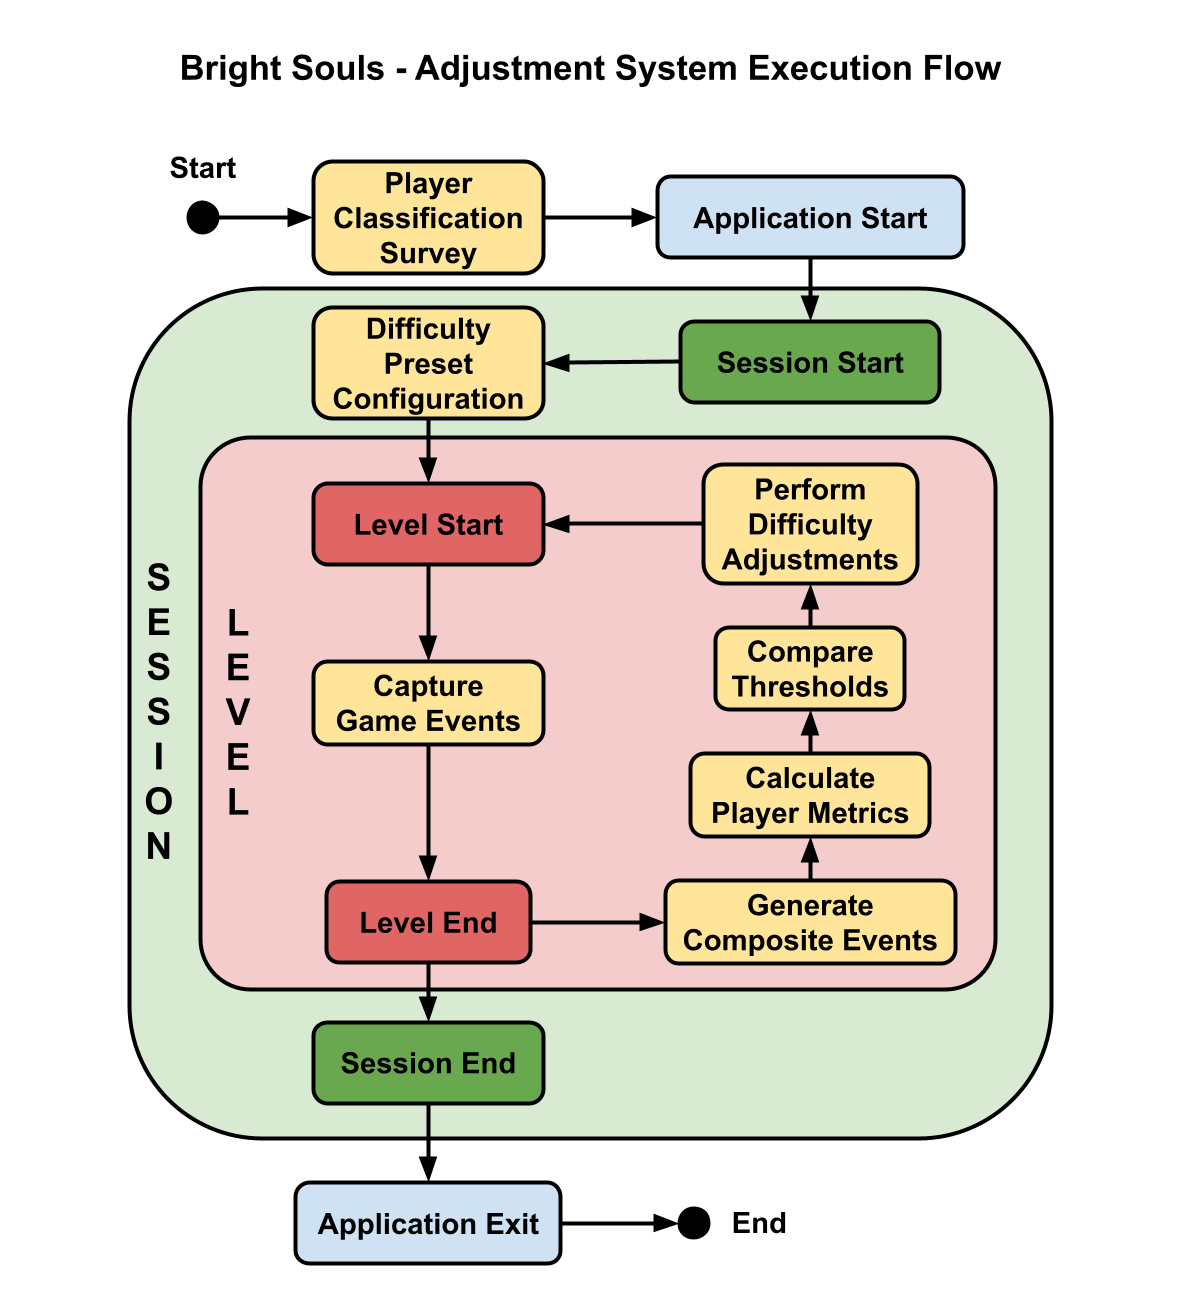
\includegraphics[width=34em]{figures/fig-adjustments-execution-flow.png}
        \legend{Source: Diagram assembled by authors.}
        \label{fig:adjustments-execution-flow}
    \end{center}
\end{figure}

We can start to define player \emph{profile} and \emph{performance} by implementing a pipeline of data acquisition, manipulation and analysis using a log of \emph{Events} raised during a play session. To do this, we implement a set of components that observe the actions performed by in-game entities to raise parametrized events while also gathering variable elements of contextual data as input.

Events are then packaged into a standardized data structure called \textsc{EventInstance}, where we store data such as a \emph{Timestamp} which represents the time since application start where an event was raised, a \emph{Name} which is used as an identifier for the event, a \emph{Type} which is used to determine the superset of systems where the event is raised, a \emph{Source} which is used to determine which in-game entity the event is related to, and a set of \emph{Parameters} which are valued types that might contain contextual data for the event. Table \ref{tab:event-instance} shows a detailed description of the fields in the \textsc{EventInstance} data structure, along with the associated types for each fields.

% * Table: Event Instances
% Event Instance
%   • Timestamp ( Time : double )
%   • Name ( String )
%   • Type ( String )
%   • Source ( ObjectId : GUID )
%   • Params[]
%       • { "name", "type", "value" }

\begin{table}
    \begin{center}
      \caption{A description of the fields associated with an \textsc{EventInstance}.}
      \label{tab:event-instance}
      \rowcolors{2}{}{gray!25} % Alternate row colors
      \begin{tabular}{ >{\small}w{l}{5em} m{7em} m{16em} } % alignments and column size
        \addlinespace
        \toprule
        % Headings
        \bf Field Name & \bf Field Type  & \bf Description \\
        \midrule
        % Data
        Timestamp      & double          & The time since application start when an event was 
                                           raised. Measured in seconds.                        \\
        Name           & String          & The Name Identifier for an event.                   \\
        Type           & String          & The System from which the event is raised from.     \\
        Source         & ObjectId        & The source in-game entity which caused the event to 
                                           be raised.                                          \\
        Params         & Array of Tuples & A set of data parameters, given in string format,  
                                           that are used to represent any contextual related 
                                           with the event.                                     \\
        \bottomrule
      \end{tabular}
    \end{center}
\end{table}

% - Write events to file in batches for performance
Events are captured and written to output files in batches to minimize performance costs over extended gameplay sessions. By doing this, frame rendering "hiccups" are minimized to a few particular moments where events exceed a specific threshold of allocated memory for batches, and in most instances do not occur over the duration of a game level. We attempt to keep the use of the input/output system and any data processing restricted to the duration of the loading screen, which happens in the transition between in-game levels. Since players does not have any sort of input or control over the application during the loading screen, this implementation abstracts the processing from the player, keeping the gameplay experience fluid.

\sepfootnotecontent{fn:play-session}{A Play Session is delimited by the moment where a user starts the game application and the moment where the user exits the application, returning to the operating system.}

% - Events are stored in a simple .csv file
% - .csv file is uploaded to google sheets after session
For each \emph{Play Session}\sepfootnote{fn:play-session}, we store a unique \emph{CSV} (Comma-Separated Values) file that is implemented to serve as a simplified relational database to store in-game events. Before the end of a play session and after all levels are completed by the player, our database files are uploaded to a \emph{Google Sheets} repository using the \emph{Sheets API}.

\subsection{Captured Events}

In this section, we specify the basic events that are captured in the data acquisition step of our performance tracking pipeline. First, we explain the difference between \emph{discrete} events and \emph{timer-based} events, which are both part of the \emph{basic events} category. After collecting events over the course of a play session or level, we aggregate and transform basic events into \emph{composite events}, which are abstractions used to simplify our definitions for metrics.

% ========================================
%  Base Events
% ========================================

% Event types
%   - Raised, Timer-based, Composite
Discrete events are events that can be raised at any given moment in a session. They do not have a pre-defined time-based restriction, and instead are simply raised from signals emitted from entity components. An example of a discrete event would be the player character performing an attack, where the occurrence of the event depends entirely on input provided by the player and can not be bound to any specific timed measure. Discrete events are generally used to represent system-based state changes, entity actions and the results of actions. In table \ref{tab:discrete-events}, we specify the discrete events in our implementation.

% * Table - Discrete Events
% TODO Table - Discrete Events
%
%   Game Loop
%       • Session Started
%           • { "sessionId" , GUID  }
%       • Session Ended
%           • { "sessionId" , GUID  }
%       • Level Started
%           • { "levelNumber" , int  }
%           • { "levelLayout" , GUID }
%       • Level Ended
%           • { "levelNumber" , int  }
%           • { "levelLayout" , GUID }
%   Encounter
%       • Encounter Started
%           • { "encounterId" , GUID  }
%       • Encounter Ended
%           • { "encounterId" , GUID  }
%       • Entity Entered Encounter
%           • { "encounterId" , GUID  }
%   Action
%       • Attack Start
%           • { "attackId" , "GUID" }
%       • Attack End
%           • { "attackId" , "GUID" }
%       • Block Start
%       • Block End
%       • Dodge Start
%           • { "position"  , "Vector3" }
%           • { "direction" , "Vector3" }
%       • Dodge End
%           • { "position"  , "Vector3" }
%   Response
%       • Hit Entity
%           • { "target" , "GUID"  }
%           • { "damage" , "float" }
%       • Hit by Entity 
%           • { "attacker" , "GUID"  }
%           • { "damage"   , "float" }
%       • Blocked Attack
%       • Dodged Attack
%       • Staggered
%       • Death

\begin{table}
    \begin{center}
      \caption{A list of the discrete events captured over a play session in our implementation.}
      \label{tab:discrete-events}
      \rowcolors{2}{}{gray!25} % Alternate row colors
      \begin{tabular}{ w{l}{7em} m{6em} w{l}{9em} m{10em} } % alignments and column size
        \addlinespace
        \toprule
        % Headings
        \bf Name & \bf Category & \bf Parameters & \bf Description \\
        \midrule
        % Game System Events
        Session Start & GameSystem & sessionId : GUID & User started and loaded the application. \\
        Session End   & GameSystem & sessionId : GUID & User quit the application. \\
        Level Start   & GameSystem & \makecell[l]{levelNumber : int\\levelLayout : GUID} & Player started a level. \\
        Level End     & GameSystem & \makecell[l]{levelNumber : int\\levelLayout : GUID} & Player finished level. \\
        \midrule
        % Encounter Events
        Encounter Start & Encounter & encounterId : GUID & User started and loaded the application. \\
        Encounter End   & Encounter & encounterId : GUID & User started and loaded the application. \\
        \makecell[l]{Entity Enter\\Encounter} & Encounter & encounterId : GUID & User started and loaded the application. \\
        \midrule
        % Action Events
        \midrule
        % Response Events
        \bottomrule
      \end{tabular}
    \end{center}
\end{table}

In contrast, timer-based events are raised repeatedly after fixed time intervals over the course of a level or play session. They are generally used to track values and actions that change over the course of time, such as the position of an entity, the movement performed by the player and the proximity of the player to walls and obstacles. Contrary to discrete events, timer-based events use a \emph{polling} approach to determine the value of its parameters, instead of the signal-based system used by discrete events. In table \ref{tab:timer-based-events}, we specify the timer-based events used in our implementation.

% * Table - Timer-Based Events
%
%   • Entity Position
%       • Global Position (Vector3)
%   • Entity Movement
%       • Distance (float)
%       • Direction (Vector3)

\begin{table}[!ht]
    \begin{center}
      \caption{A list of the timer-based events captured in our implementation.}
      \label{tab:timer-based-events}
      \rowcolors{2}{}{gray!25} % Alternate row colors
      \begin{tabular}{ >{\small}w{l}{4em} >{\small}w{c}{3em} >{\small}w{c}{4.5em} >{\small}w{c}{2.5em} >{\small}m{15em} } % alignments and column size
        \addlinespace
        \toprule
        % Headings
        \bf Name & \bf Category & \bf Params & \bf Types & \bf Description \\
        \midrule
        % Entity Events
        Position & Entity & position & Vector3 & The position of an entity at a given time. \\
        \midrule
        Movement & Player & \makecell[c]{distance\\direction} & \makecell[c]{float\\Vector3} & The movement performed by the player in a small time frame. \\
        Health   & Player & value & float & The Health of the Player at a given time. \\
        Stamina  & Player & value & float & The Stamina of the Player at a given time. \\
        \makecell[l]{Available\\Dodge Area} & Player & value & float & The percentage of the area where the player is able to dodge that is not occupied by walls or other obstacles. \\
        \bottomrule
      \end{tabular}
    \end{center}
\end{table}

% Composite Events
%   - Use of composite events as helpers
%   - Composite events are runtime only
The last type of events implemented in our application are the \emph{composite} events, which are created by aggregating discrete and timer-based events and are used as helper tools to simplify the definition of our metrics. Composite events are not raised or stored during play sessions, as they are purposed simply for the calculation of player metrics. Composite events are generated between and after levels, before metric calculation and dynamic difficulty adjustments take place, and only exist at runtime.

The aggregation of basic events into composite events uses the \emph{Timestamp} and \emph{Parameters} of events to establish the correlation between events and guarantee that events of different scopes are not being used to calculate the same metric. For instance, the \emph{Successful Block} event uses the parameter \emph{AttackId} from \emph{AttackStart} events to check if the attack being blocked is the same attack that initiated right before or after the player started blocking. Table \ref{tab:composite-events} specifies the composite events used in our implementation. 

% * Table - Composite Events
% * Table - Composite events

\begin{table}[!ht]
    \begin{center}
      \caption{A list of the composite events that are created by aggregating basic events.}
      \label{tab:composite-events}
      \rowcolors{2}{}{gray!25} % Alternate row colors
      \begin{tabular}{ >{\small}w{l}{4em} >{\small}w{c}{4em} >{\small}w{c}{10em} >{\small}m{12em} } % alignments and column size
        \addlinespace
        \toprule
        % Headings
        \bf Name & \bf Category & \bf Base Events & \bf Description \\
        \midrule
        % Session Composite Events
        \makecell[l]{Encounter\\Completed} & Game & \makecell[c]{EncounterStart\\EncounterEnd} & Player successfully eliminated all enemies in an encounter. \\
        \makecell[l]{Level\\Completed} & Game & \makecell[c]{LevelStart\\LevelEnd} & Player successfully completed a level. \\
        \makecell[l]{Session\\Completed} & Game & \makecell[c]{SessionStart\\SessionEnd} & Player finished a play session. \\
        \midrule
        % Combat Composite Events
        \makecell[l]{Successful\\Dodge} & Combat & \makecell[c]{AttackStart,DodgeStart\\!HitByEntity,AttackEnd} & Player successfully dodged an attack. \\

        \makecell[l]{Failed\\Dodge} & Combat & \makecell[c]{AttackStart,DodgeStart\\HitByEntity,AttackEnd} & Player failed to dodge an attack. \\

        \makecell[l]{Successful\\Block} & Combat & \makecell[c]{AttackStart,BlockStart\\BlockedAttack,AttackEnd} & Player successfully blocked an attack. \\

        \makecell[l]{Failed\\Block} & Combat & \makecell[c]{AttackStart,BlockStart\\HitByEntity,DefenseBreak\\AttackEnd} & Player failed to block an attack. \\

        \makecell[l]{Successful\\Avoid} & Combat & \makecell[c]{AttackStart,!HitByAttack\\!BlockStart,!DodgeStart\\AttackEnd} & Player successfully avoided an attack without performing a Dodge or Block. \\

        \makecell[l]{Failed\\Avoid} & Combat & \makecell[c]{AttackStart,HitByAttack\\!BlockStart,!DodgeStart\\AttackEnd} & Player got hit by an attack without performing a Dodge or Block. \\

        \makecell[l]{Offensive\\Action} & Combat & \makecell[c]{AttackStart} & Player performed an offensive action. \\

        \makecell[l]{Defensive\\Action} & Combat & \makecell[c]{DodgeStart,BlockStart\\SuccessfulAvoid} & Player performed a defensive action. \\

        \midrule
        % Entity Composite Events
        \makecell[l]{Entity\\Eliminated} & Entity & \makecell[c]{EncounterStart\\EntityJoinEncounter\\EntityDeath} & Player eliminates an entity after it joins an encounter \\
        \bottomrule
      \end{tabular}
    \end{center}
\end{table}

% TODO Table - Composite Events

%   • Successful Dodge
%       • Attack Start (Enemy)
%       • Dodge Start (Player)
%       • NOT HitByAttack (Player)
%       • Attack End (Enemy)
%   • Failed Dodge
%       • Attack Start (Enemy)
%       • Dodge Start (Player)
%       • Hit By Entity
%       • Attack End (Enemy)
%   • Successful Block
%       • Attack Start (Enemy)
%       • Block Start (Player)
%       • Blocked Attack (Player)
%       • Attack End (Enemy)
%   • Failed Block
%       • Attack Start (Enemy)
%       • Block Start (Player)
%       • Hit By Entity OR Defense Break
%       • Attack End (Enemy)
%   • Successful Avoid
%       • Attack Start (Enemy)
%       • NOT Hit By Attack (Player)
%       • Attack End (Enemy)
%   • Failed Avoid
%       • Attack Start (Enemy)
%       • NOT Block Start (Player)
%       • NOT Dodge Start (Player)
%       • Attack End (Enemy)

\subsection{Player Metrics}

After the player successfully completes a level and we perform aggregation of basic events into composite events, we can begin to calculate the metrics which will be used as input to perform difficulty adjustments. Since reading and performing data transformations over events in our application requires a high processing and \emph{Input/Output} load, we chose to implement calculation of player metrics in non-interactive segments of our application. This imposes a limitation of our application being unable to perform difficulty adjustments in real time. Instead, adjustments are performed on a per-level basis, with metrics being calculated before each level is started.

We use our previously defined adjustments as a basis to define which metrics would be gathered. Metrics are meant to evaluate the efficiency and tendencies of a player. Each difficulty adjustment relates to one or several aspects of the decision-making process and skill level of a player, and thus metrics are used to provide an estimation of the efficiency of player decisions or their ability to execute the appropriate actions for each situation.

In our implementation, we categorize metrics into \emph{profile} and \emph{performance metrics}. Profile metrics have the purpose of identifying player habits and common responses to the environment or encounters, as seen in \cite{ARTICLE_DynamicPlayerModelling}. In general, profile metrics in our implementation are used to make the game more challenging and interesting, providing a variety to actions performed by enemies and enemy positioning setups for encounters in the later levels.

We use profile metrics to detect the frequency of defensive actions and target prioritization tendencies. The information provided by the player profile is then used to modify the chance of enemies performing a specific action and their placement in levels.  Table \ref{tab:profile-metrics} provides a list of the profile metrics implemented in our application, along with the events that are used to calculate each metric and a brief description of its purpose.

% * Table - Profile Metrics
% * Table - Profile Metrics

\begin{table}[!ht]
    \begin{center}
      \caption{A list of the \emph{profile metrics} implemented to monitor player habits and common responses to combat situations in our application.}
      \label{tab:profile-metrics}
      \rowcolors{2}{}{gray!25} % Alternate row colors
      \begin{tabular}{ >{\small}w{l}{4.5em} >{\small}w{c}{7em} >{\small}m{16.5em} } % alignments and column size
        \addlinespace
        \toprule
        % Headings
        \bf Name & \bf Related Events & \bf Description \\
        \midrule

        \makecell[l]{Block\\Frequency} & \makecell[c]{SuccessfulBlock\\FailedBlock\\DefensiveAction} & The frequency [0,1] in which the player performs the Block action in comparison to other defensive methods. \\

        \makecell[l]{Dodge\\Frequency} & \makecell[c]{SuccessfulDodge\\FailedDodge\\DefensiveAction} & The frequency [0,1] in which the player performs the Dodge action in comparison to other defensive methods. \\

        \makecell[l]{Avoid\\Frequency} & \makecell[c]{SuccessfulAvoid\\DefensiveAction} & The frequency [0,1] in which the player avoids an attack without blocking or dodging in comparison to other defensive methods. \\

        \makecell[l]{Avg. Enemy\\Lifetime} & \makecell[c]{EncounterStart\\EntityJoinEncounter\\EntityDeath} & The average time it takes for an enemy to die from the moment it joins an encounter. This metric has one instance per enemy type. \\

        \bottomrule
      \end{tabular}
    \end{center}
\end{table}

% Profile

%   Defensive action frequency
%       • Blocking frequency
%       • Dodge frequency
%       • Avoid frequency

%   • Enemy Lifetime
%       - Per enemy lifetime
%       - Scoped in {Encounter, Level, Session}

% Performance Metrics

In contrast, performance metrics gather the results of player actions, focusing on measuring success, failure and efficiency of the execution of game mechanics and the player decision-making process. We attempt to use performance metrics to smooth out the learning curve for beginner players, while also providing more challenging situations and behaviors for veteran players.

Some examples of adjustments performed using performance metrics include the number of enemies that can simultaneously attack the player, visual cues for enemy attacks, the frequency of checkpoints in levels and the overall game speed. Table \ref{tab:performance-metrics} provides a list of the performance metrics implemented in our application, specifying the events used to calculate them and a brief description of their purpose.

% * Table - Performance Metrics
\begin{table}[!ht]
    \begin{center}
      \caption{A list of the \emph{performance metrics} implemented to perform adjustments related to the efficiency and results of player actions.}
      \label{tab:performance-metrics}
      \rowcolors{2}{}{gray!25} % Alternate row colors
      \begin{tabular}{ >{\small}w{l}{4.5em} >{\small}w{c}{7em} >{\small}m{16.5em} } % alignments and column size
        \addlinespace
        \toprule
        % Headings
        \bf Name & \bf Related Events & \bf Description \\
        \midrule

        \makecell[l]{Level\\Duration} & \makecell[c]{LevelStart\\LevelEnd} & The time it takes for the player to clear a level. \\

        \makecell[l]{Encounter\\Duration} & \makecell[c]{EncounterStart\\EncounterEnd} & The time it takes for the player to eliminate all enemies in an encounter. \\

        \makecell[l]{Session\\Duration} & \makecell[c]{SessionStart\\SessionEnd} & The time it takes for the player to complete all levels in a game session. \\

        \midrule

        \makecell[l]{Dodge\\Efficiency} & \makecell[c]{SuccessfulDodge\\FailedDodge} & The rate of successful dodges in relation to the total number of performed dodges. \\

        \makecell[l]{Block\\Efficiency} & \makecell[c]{SuccessfulBlock\\FailedBlock} & The rate of successfully performed blocks in relation to the total number of blocks. \\

        \makecell[l]{Avoid\\Efficiency} & \makecell[c]{SuccessfulAvoid\\FailedAvoid} & The rate of attacks successfully avoided without blocking or dodging. \\

        \makecell[l]{Attack\\Avoidance\\Efficiency} & \makecell[c]{Successful\\and Failed Blocks,\\Dodges,Avoids} & The rate of attacks that are successfully blocked, dodged or avoided in comparison to attacks that hit the player. \\

        \makecell[l]{Obstacle\\Avoidance} & \makecell[c]{Available\\Dodge Area} & The average percentage of the dodge area that is occupied by walls and obstacles over the course of a Level. \\

        \midrule

        \makecell[l]{Avg. Health\\Level} & \makecell[c]{Health\\AttributeChanged} & The average Health level of the player over the course of an Encounter or Level. \\

        \makecell[l]{Avg. Stamina\\Level} & \makecell[c]{Stamina\\AttributeChanged} & The average Stamina level of the player over the course of an Encounter or Level. \\

        \makecell[l]{Avg. Health\\Lost Per\\Encounter} & \makecell[c]{EncounterStart\\AttributeChanged\\EncounterEnd} & The average Health lost by the player over the course of an Encounter. \\

        \makecell[l]{Number of\\Deaths} & \makecell[c]{EncounterStart\\LevelStart,Death} & The number of times the player died over the curse of an Encounter or a Level. \\

        \makecell[l]{Average\\Deaths} & \makecell[c]{LevelStart\\Death} & The average number of times the player died over the course of a Session. \\

        \midrule

        \makecell[l]{Avg. Time\\To Kill} & \makecell[c]{AttackStart\\Death} & The average time for the player to kill an enemy type since the first attack hits. \\

        \makecell[l]{Atk. Window\\Efficiency} & \makecell[c]{CooldownStart\\HitEntity\\CooldownEnd} & The average damage dealt by the player during an attack window opportunity where an enemy is in cooldown. \\

        \bottomrule
      \end{tabular}
    \end{center}
\end{table}

% Performance Metrics List

%   • Level Duration
%       • Level Start
%       • Level End

%   • Encounter Duration
%       • Encounter Start
%       • Encounter End

%   • Session Duration
%       • Session Start
%       • Session End

%   Level Clear Time
%       • Level Duration

%   Health efficiency
%	    • Average health lost per {Encounter, Level}

%   Action Efficiency
%       • Blocking Efficiency
%       • Dodge Efficiency
%       • Avoid Efficiency
%   Stamina Management Efficiency
%       • Average Stamina Level
%       • Average Stamina When Initiating Attack Sequence
%       • Average Stamina Level during encounter
%   Damage dealing efficiency
%       • Attack Window Efficiency
%       • Attack Sequence Average Damage
%   Positional Efficiency
%       • Obstacle Avoidance

% • Attack Avoidance Efficiency
%   - Successful Dodges + Blocks + Avoids / Failed Dodges + Blocks + Avoids
%   - Scoped in Encounter, Level, Session

% ============================================================================
% ============================================================================
% ============================================================================

\section{Difficulty Adjustments}
\label{sec:adjustments}

% Difficulty as an N-dimensional set of parameters
% Parameters are adjusted using one or more metrics
In our implementation, we treat difficulty as an N-dimensional set of parameters that are adjusted according to player profile and performance. Each difficulty parameter is adjusted based on a subset of the metrics we defined previously. Therefore, each metric can be mapped to one or more adjustments, and conversely each adjustment is influenced by one or more metrics.

% We chose the statistical model approach because it can better represent the process of game development in the video game industry, where values and thresholds for difficulty adjustments can be tested and adjusted through iterative play-testing sessions.
The purpose of our experiment is to compare N-dimensional difficulty to the definition of difficulty as multiple preset configurations of all adjustment parameters. Therefore, we found that representing adjustments through a probabilistic model, as explored in section \ref{sec:statistical-adjustments} is best suited to represent the nature of the game development process in the video game industry. During the game development process, game designers perform iterative play-testing sessions, where users are monitored to identify flaws in game design or adjustable properties that might better represent the desired outcome of in-game systems. Through the same philosophy, we can incorporate the probabilistic model in the game design process, where values and thresholds for difficulty adjustments can be tested and adjusted through the iterative play-testing sessions to better represent the desired learning and challenge curve adjustment for the game.

% Discrete values for parameters, switched between by thresholds
% Thresholds gathered with iterative play sessions
% Metrics were clustered manually to create thresholds
We define discrete values to each parameter, which are switched between based on thresholds applied over player metrics. The thresholds were gathered by performing iterative play sessions with players from multiple skill levels and analyzing the data for the metrics over different types of players and different difficulty levels. We attempted to cluster the values gathered from metrics manually, where we separated users by their reported previous experience with games, and specifically with Souls-like entries. Details on how thresholds for adjustments were gathered are further specified in section \ref{sec:experiment-methodology}.

% Adjustments occur in multiple subsystems
% Adjustments created by analyzing the aspects and difficulty of Dark Souls
The adjustments in our implementation are scoped within multiple game subsystems, and were elected based in the considerations discussed in section \ref{sec:pain-points-dark-souls}. Each parameter is adjusted within a progressive set of values, where at least one of the values would be best suited to an inexperienced player and another would be designed for a veteran of the Souls-like genre. Table \ref{tab:adjustments} lists the adjustments included in our implementation, including their name, the metrics that are related to them and a brief description of their purpose.

% * Table - Adjustments
% * Table - Adjustments

\begin{table}[!ht]
    \begin{center}
      \caption{A list of the \emph{adjustments} that were implemented in our application to define game difficulty as an N-dimensional set of parameters.}
      \label{tab:adjustments}
      \rowcolors{2}{}{gray!25} % Alternate row colors
      \begin{tabular}{ >{\small}w{l}{5.5em} >{\small}w{c}{7em} >{\small}m{20em} } % alignments and column size
        \addlinespace
        \toprule
        % Headings
        \bf Name & \bf Related Metrics & \bf Description \\
        \midrule

        \makecell[l]{Pierce Attack\\Chance Mod.} & \makecell[c]{Block Efficiency\\Block Frequency} & The modifier for the chance of an enemy performing a \emph{Pierce} attack. \\

        \makecell[l]{Sweep Attack\\Chance Mod.} & \makecell[c]{Dodge Efficiency\\Dodge Frequency} & The modifier for the chance of an enemy performing a \emph{Sweep} attack. \\

        \makecell[l]{Charge Attack\\Chance Mod.} & \makecell[c]{Avoid Efficiency\\Avoid Frequency} & The modifier for the chance of an enemy performing a \emph{Charge} attack when the player is out of attack range. \\

        \midrule

        \makecell[l]{Near Target\\Max. Number} & \makecell[c]{Attack Avoidance\\Efficiency\\Avg. Stamina Level} & The number of enemies that can be in close quarters (near the player) in an encounter. \\

        \makecell[l]{Simultaneous\\Max. Attacks} & \makecell[c]{Attack Window\\Efficiency\\Avg. Health Lost\\Per Encounter} & The number of enemies that can simultaneously attack the player in an encounter. \\

        \makecell[l]{Global Atk.\\Cooldown} & \makecell[c]{Attack Window\\Efficiency} & The global cool-down timer for all enemy agents after an attack is performed by any agent. The number of simultaneous attacks defines the number of separate timers. \\

        \makecell[l]{Global Special\\Atk. Cooldown} & \makecell[c]{Attack Avoidance\\Efficiency} & The global cool-down timer for all enemy agents after a Special Attack is performed by any agent. \\

        \midrule

        \makecell[l]{Game Speed} & \makecell[c]{Attack Avoidance\\Efficiency} & The global \emph{Timescale} at which the game runs, which is increased or decreased according to the effectiveness of player reactions to combat situations. \\

        \makecell[l]{Attack\\Visual Cues} & \makecell[c]{Attack Avoidance\\Efficiency} & The presence or absence of easily recognizable Attack Startup Animations indicating which attack an enemy is performing. \\

        \midrule

        \makecell[l]{Archer Enemy\\Placement} & \makecell[c]{Avg. Archer\\Lifetime} & The general positional placement of archer enemies in levels so that they are easier or harder to eliminate during combat encounters. \\

        \makecell[l]{Basic Enemies\\Occurence} & \makecell[c]{Avg. Enemy\\Lifetime} & The chance of a Basic Enemy using one of the available slots for enemy placement in the level layout to be placed in an encounter. \\

        \makecell[l]{Warrior Enemies\\Occurence} & \makecell[c]{Avg. Non-Warrior\\Lifetime} & The chance of a Warrior Enemy using one of the available slots for enemy placement in the level layout to be placed in an encounter. \\

        \makecell[l]{Knight Enemies\\Occurence} & \makecell[c]{Avg. Health Lost\\Per Encounter\\Attack Window\\Efficiency} & The chance of a Knight Enemy using one of the available slots for enemy placement in the level layout to be placed in an encounter. \\

        \midrule

        \makecell[l]{Combat Area\\Openness} & \makecell[c]{Obstacle Avoidance} & The size and placement of obstacles in areas where combat encounters are designed to occur. \\

        \makecell[l]{Checkpoint\\Placement} & \makecell[c]{Level Duration\\Avg. Deaths/Level} & The presence or absence of checkpoints in specific areas of levels, such as at a central point of level layouts or right before combat encounters. \\

        \bottomrule
      \end{tabular}
    \end{center}
\end{table}

% Enemy Individual Behavior
% 	• Special Attacks
% 		○ Pierce attack chance
% 			§ Blocking Efficiency
% 			§ Blocking Frequency
% 		○ Charge attack chance
% 			§ Avoid Efficiency
% 			§ Avoid Frequency
% 		○ Sweep attack chance
% 			§ Dodge Efficiency
% 			§ Dodge Frequency

% Enemy Group Behavior
% 	• Number in close quarters
% 		○ {1, 2, 3} enemies
% 		○ Attack Avoidance Efficiency
% 		○ Avg. Stamina Level
% 	• Simultaneous attacks
% 		○ {1, 2} attacks
% 		○ Attack Window Efficiency
% 		○ Avg. Health Lost per Encounter
% 	• Global Attack Cooldown
% 		○ {5, 4.4, 3.5} seconds
% 		○ Attack Window Efficiency
% 	• Global Special Attack cooldown
% 		○ {10, 8, 6} seconds
% 		○ Attack Window Efficiency
%       ○ Attack Avoidance Efficiency

% Accessibility
%	• Game Speed
%		○ {0.8, 0.9, 1.0} speed
%		○ Attack Avoidance Efficiency
%	• Attack Visual Cues
%		○ Red highlight on attack
%		○ Default attack anims
%       ○ Ambiguous animations

% Encounter design
%	• Archer enemy placement
%		○ Forward positions
%		○ Backline positions
%		○ Long-range positions
%		○ Avg Archer Lifetime
%	• Basic enemies occurrence
%		○ Avg Archer Lifetime
%	• Warrior enemies occurrence
%		○ Avg Non-Warrior Lifetime
%	• Knight enemies occurrence
%		○ Attack Avoidance Efficiency
%		○ Damage Efficiency

% Level Design
%	• Combat area openess
%		○ Wide open areas
%		○ Mid-sized with obstacles
%		○ Constricted areas
%		○ Level Clear Time
%		○ Deaths
%	• Checkpoints
%		○ One checkpoint per encounter
%		○ Mid level checkpoints
%		○ Single level checkpoint


% We use three difficulty presets as a base to perform adjustments on.
% Each preset defines values for all adjustable parameters.
As a base guideline to define the discrete values for parametrized adjustments, and to define the thresholds that are compared to metrics to perform such adjustments, we attempt to define three base difficulty presets which contain value definitions for all adjustments parameters based on classification of player profile and skill levels. The base presets for adjustment values are assigned at the beginning of a session, and the preset is initially assigned to a player based on a \emph{Player Classification Survey}, which is further detailed at section \ref{sec:experiment-methodology}.

% Base presets define difficulty as a one dimensional configuration
% As session progresses, parameters start to diverge
Through the base presets, we are initially defining game difficulty as a one dimensional configuration of multiple parameters. However, as a session progresses and we capture in-game events and calculate performance and profile metrics, we can begin to compare such metrics to a set of thresholds that were previously defined, and certain parameters will begin to be adjusted independently and diverge, effectively transforming game difficulty into an N-dimensional set of parameters.

% The thresholds are not a continuous set of values, meaning that the conditions for each threshold are not always valid
% If the conditions are not met, the adjustment parameter is kept the same
% This works because of the initial parameters defined by player classification survey
It is important to note that the thresholds defined for each parameter value do not represent a continuous group of validation conditions, meaning that it is not guaranteed that the metrics captured from the player will be necessarily validated against any of the threshold conditions for a parameter. This is done by design so that if the conditions for all thresholds of a parameter are not met, the adjustment parameter is kept the same. Therefore, the transition conditions for a lower parameter value to be adjusted into a higher value can not be symmetrically inverted as to adjust the higher value into the lower value, which generates a tendency for the player to be kept in the same difficulty level unless their performance or profile metrics relevantly deviate from the intended user group.

% Table detailing thresholds and values for adjustments
In table \ref{tab:adjustment-thresholds} we attempt to organize  and specify the values that parametrized adjustments can be assigned to and their associated metrics, along with the threshold values for each metric. Some of the adjustment parameters have restricted value ranges with the purpose of making the game more difficult or easier than the proposed core experience of our game, and will present a default value as a minimum or maximum limit which represents the standard experience for an average skilled player. For this purpose, we attempt to visually separate adjustments in regions that describe their target player profile stereotype.

% * Table - Adjustments

\begin{table}[!ht]
    \begin{center}
      \caption{A list of the thresholds and their associated values for each parametrized difficulty adjustment in our application.}
      \label{tab:adjustment-thresholds}
      \rowcolors{2}{}{gray!25} % Alternate row colors
      \begin{tabular}{ >{\small}w{l}{5.5em} >{\small}w{c}{7em} >{\small}w{c}{2.5em} >{\small}w{c}{9.5em} >{\small}w{c}{6em} } % alignments and column size
        \addlinespace
        \toprule
        % Headings
        \bf Name & \bf Parameters & \bf Symbol & \bf Thresholds & \bf Values \\
        \midrule

        \makecell[l]{Pierce Attack\\Chance Mod.} & \makecell[c]{BlockEff\\BlockFreq} & \makecell[c]{BE\\BF} & \makecell[c]{BE < 0.3, BF < 0.5\\BE > 0.3, BF > 0.2\\BE > 0.6, BF > 0.5} & \makecell[c]{0.5x\\1.0x\\1.35x} \\

        \makecell[l]{Sweep Attack\\Chance Mod.} & \makecell[c]{DodgeEff\\DodgeFreq} & \makecell[c]{DE\\DF} & \makecell[c]{DE < 0.3, DF < 0.5\\DE > 0.3, DF > 0.2\\DE > 0.6, DF > 0.5} & \makecell[c]{0.5x\\1.0x\\1.35x} \\

        \makecell[l]{Charge Attack\\Chance Mod.} & \makecell[c]{AvoidEff\\AvoidFreq} & \makecell[c]{AE\\AF} & \makecell[c]{AE < 0.3, AF < 0.5\\AE > 0.3, AF > 0.2\\AE > 0.6, AF > 0.5} & \makecell[c]{0.5x\\1.0x\\1.35x} \\

        \midrule

        \makecell[l]{Near Target\\Max. Number} & \makecell[c]{AtkAvoidanceEff\\AvgStaminaLevel} & \makecell[c]{AAE\\ASL} & \makecell[c]{AAE < 0.4\\AAE > 0.4, ASL < 0.6\\AAE > 0.6, ASL > 0.4} & \makecell[c]{1 Agent\\2 Agents\\3 Agents} \\

        \makecell[l]{Simultaneous\\Max. Attacks} & \makecell[c]{AtkWindowEff\\AvgHealthLostEnc} & \makecell[c]{AWE\\AHLE} & \makecell[c]{AWE < 0.1\\AWE > 0.15, AHLE < 50} & \makecell[c]{1 Attack\\2 Attacks} \\

        \makecell[l]{Global Atk.\\Cooldown} & \makecell[c]{AtkWindowEff} & \makecell[c]{AWE}  & \makecell[c]{AWE < 0.1\\AWE > 0.15, AWE < 0.18\\AWE > 0.225} & \makecell[c]{6 seconds\\4.5 seconds\\3.5 seconds} \\

        \makecell[l]{Global Special\\Atk. Cooldown} & \makecell[c]{AtkAvoidanceEff} & \makecell[c]{AAE}  & \makecell[c]{AAE < 0.3\\AAE > 0.3, AAE < 0.45\\AAE > 0.6} & \makecell[c]{11 seconds\\9 seconds\\7.5 seconds} \\

        \midrule

        \makecell[l]{Game Speed} & \makecell[c]{AtkAvoidanceEff} & \makecell[c]{AAE}  & \makecell[c]{AAE < 0.15\\AAE < 0.25\\AAE > 0.25} & \makecell[c]{0.85x\\0.925x\\1.0x} \\

        \makecell[l]{Attack\\Visual Cues} & \makecell[c]{AtkAvoidanceEff} & \makecell[c]{AAE}  & \makecell[c]{AAE < 0.2\\AAE > 0.2, AAE < 0.6\\AAE > 0.6} & \makecell[c]{Red Highlight\\Normal\\Ambiguous} \\

        \midrule

        \makecell[l]{Archer Enemy\\Placement} & \makecell[c]{AvgArcherLife} & \makecell[c]{AAL} & \makecell[c]{AAL > 40s\\AAL > 25s\\AAL < 10s} & \makecell[c]{Frontline\\Rearguard\\Long-Range} \\

        \makecell[l]{Basic Enemies\\Occurence} & \makecell[c]{AvgEnemyLife} & \makecell[c]{AEL}  & \makecell[c]{AEL > 30s\\AEL < 25s} & \makecell[c]{Normal\\Additional} \\

        \makecell[l]{Warrior Enemies\\Occurence} & \makecell[c]{AvgNonWarriorLife} & \makecell[c]{ANWL}  & \makecell[c]{ANWL > 30s\\ANWL < 25s} & \makecell[c]{Normal\\Additional} \\

        \makecell[l]{Knight Enemies\\Occurence} & \makecell[c]{AvgHealthLostEnc\\AtkWindowEff} & \makecell[c]{AHLE\\AWE} & \makecell[c]{AHLE > 40, AWE < 0.15\\AHLE < 40, AWE > 0.15} & \makecell[c]{Normal\\Additional} \\

        \midrule

        \makecell[l]{Combat Area\\Openness} & \makecell[c]{ObstacleAvoidance} & \makecell[c]{OA} & \makecell[c]{OA < 0.7\\OA > 0.7, OA < 0.8\\OA > 0.8} & \makecell[c]{Wide Open\\Mid-Sized\\Constricted} \\

        \makecell[l]{Checkpoint\\Placement} & \makecell[c]{AvgLevelDur\\AvgDeathsLevel} & \makecell[c]{ALD\\ADPL}  & \makecell[c]{ALD > 5min, ADPL > 7\\ALD > 4min, ADPL > 5\\ALD < 4min, ADPL < 5} & \makecell[c]{Per Encounter\\Mid Level\\Single} \\

        \bottomrule
      \end{tabular}
    \end{center}
\end{table}


% ============================================================================
% ============================================================================
% ============================================================================